\RequirePackage[T1]{fontenc}
\documentclass[journal]{IEEEtran}
\usepackage{amsmath,amssymb,mathtools}
\usepackage{booktabs}
\usepackage{graphicx}
\usepackage{multirow}
\usepackage{array}
\usepackage{url}
\usepackage{xcolor}
\usepackage{cite}
\usepackage{xspace}
\usepackage{placeins}
% Run-in paragraph headings are not numbered in the journal layout.
\setcounter{secnumdepth}{3}
% A lightweight IEEE-compatible algorithm float avoids external package
% dependencies while retaining a numbered Algorithm caption.
\makeatletter
\newcounter{algorithm}
\renewcommand{\thealgorithm}{\arabic{algorithm}}
\def\fps@algorithm{bp}
\def\ftype@algorithm{4}
\def\ext@algorithm{loa}
\def\fnum@algorithm{Algorithm~\thealgorithm}
\newenvironment{algorithm}{\@float{algorithm}}{\end@float}
\makeatother
\newcounter{algline}
\newcommand{\algreset}{\setcounter{algline}{0}}
% Put the statement in a fixed-width box so wrapped lines align with the
% statement text rather than returning to the left margin.
\newcommand{\State}[1]{%
  \stepcounter{algline}%
  \noindent\makebox[2.2em][r]{\scriptsize\thealgline:}\hspace{0.45em}%
  \parbox[t]{\dimexpr\linewidth-3.1em\relax}{#1}\par}
\newcommand{\StateCont}[1]{%
  \stepcounter{algline}%
  \noindent\hspace*{1.25em}\makebox[2.2em][r]{\scriptsize\thealgline:}\hspace{0.45em}%
  \parbox[t]{\dimexpr\linewidth-4.35em\relax}{#1}\par}
\newcommand{\StateInner}[1]{%
  \stepcounter{algline}%
  \noindent\hspace*{2.5em}\makebox[2.2em][r]{\scriptsize\thealgline:}\hspace{0.45em}%
  \parbox[t]{\dimexpr\linewidth-5.6em\relax}{#1}\par}

% Keep wide figures at the top of text pages instead of creating
% sparsely populated float-only pages.
\setcounter{dbltopnumber}{4}
\renewcommand{\dbltopfraction}{0.95}
\renewcommand{\dblfloatpagefraction}{0.85}
\setcounter{topnumber}{4}
\setcounter{totalnumber}{6}
\renewcommand{\textfraction}{0.08}
\renewcommand{\topfraction}{0.95}
\renewcommand{\floatpagefraction}{0.7}
\setlength{\dblfloatsep}{9pt plus 2pt minus 2pt}
\setlength{\dbltextfloatsep}{6pt plus 2pt minus 2pt}
\setlength{\textfloatsep}{6pt plus 2pt minus 2pt}
\setlength{\floatsep}{6pt plus 2pt minus 2pt}
\setlength{\intextsep}{6pt plus 2pt minus 2pt}
\makeatletter
\setlength{\@dblfptop}{0pt}
\setlength{\@dblfpsep}{10pt}
\setlength{\@dblfpbot}{0pt plus 1fil}
\makeatother

\newcommand{\method}{DNQ-DLC\xspace}
\newcommand{\etal}{\textit{et al.}}
\newcommand{\tabnote}[1]{%
\vspace{1.2mm}\parbox{0.96\textwidth}{\footnotesize\textit{Note:} #1}}

\begin{document}

\bstctlcite{BSTcontrol}

\title{DNQ-DLC: Dynamic-Neighbourhood Quality-Guided Deep Latent Competition for Closed-Loop Multi-Vehicle Overtaking in Autonomous Racing}

\author{Author names, affiliations, and ORCID identifiers to be inserted before submission}

\markboth{IEEE Transactions on Intelligent Transportation Systems, Manuscript for Review}%
{DNQ-DLC: Dynamic-Neighbourhood Quality-Guided Deep Latent Competition}

\maketitle

\begin{abstract}
Racing overtakes are decided within seconds, and the constraining opponent
can change in that window. DNQ-DLC is a receding-horizon planner with three
parts: a dynamic neighbourhood that rebuilds the ego-centric interaction graph
from each observation and decides which opponents enter it, an action-conditioned
world model that rolls candidate ego actions into imagined futures, and a
quality-guided score over progress, containment, interaction and stability that
ranks those futures. Over 48 matched cases per method, five draws of the DNQ-DLC
recipe complete 45.8 of 48 cases on average, against 41.0, 41.5 and 45.5 for
three world-model variants retrained on the same data, 45 for a rule expert and
at most 35.8 for three continuous-control families, and reach the strict tier
(sustained lead, no contact, on track, stable afterwards) in 20.2 cases against
17.5, 18.5 and 13.5 for the three variants, 12 for the rule expert and at most
6.4 for the continuous-control families. The strict-tier range overlaps every
variant, while the rank-gain and containment ranges are disjoint from every
comparator draw. Every draw gains more positions per case, 4.62 to 5.02, and
spends 12.4--19.9\,\% of the episode off the racing surface against 25.0--49.7\,\%
for every variant draw. The admitted set saturates at its three-slot budget, the
imagined ego position stays within 1.2~m over four steps, the planner leaves its
rule anchor in 92--93\,\% of decisions, and the shield is active on 30--46\,\% of
steps. The claims are limited to the tested simulator and vehicle counts.
\end{abstract}

\begin{IEEEkeywords}
Autonomous racing, overtaking, world models, dynamic interaction graphs,
multi-agent decision making, receding-horizon planning.
\end{IEEEkeywords}

\section{Introduction}

\IEEEPARstart{M}{ulti-vehicle} overtaking in autonomous racing is decided within a
short window. An opportunity appears when the vehicle ahead is slower at corner exit
or leaves a line open, and it closes within a few seconds, so the decisive part of
the manoeuvre is a small share of any longer episode, and rare interactions of
this kind drive test generation for automated
driving~\cite{feng2021intelligenttest,liu2024rarity}. The opponent that
constrains the manoeuvre also changes during the pass: the vehicle that sets the
initial closing strategy gives way to an alongside vehicle, or to a vehicle that
constrains the pass from a different line. A controller therefore has to rebuild its interaction
context from each new observation, estimate what a candidate action does over
the next few tenths of a second, and trade progress against track retention,
contact risk and stability. That trade-off has no free setting: an aggressive
action can secure position while removing lateral clearance, and a conservative
one can preserve containment while the passing window closes
~\cite{raji2022multivehicle,wischnewski2023tube}. Whatever the controller
chooses, it has to remain inside the capability of the vehicle at racing
speed~\cite{betz2022autonomous,wischnewski2022iac,cheng2024chassis_trajectory,cheng2025hybrid_dynamic}.

The relevant-opponent set is not a fixed list. A leading vehicle may set the
initial closing strategy, an adjacent vehicle may define the corridor that is
open, and a vehicle that was far away can become the binding
constraint after it brakes or abandons a pass
~\cite{huang2023gameformer,sun2022intersim}. A controller that keeps a fixed
set of interaction objects, or assigns roles once and reuses them, will keep
reasoning about an opponent that no longer matters while ignoring the vehicle
that does.

Four lines of work bear on this problem. Dynamics-aware racing planners enforce
track and vehicle limits, but usually over predefined opponents or pairwise
roles~\cite{betz2023tum,jung2023kaist}. Learned policies produce nonlinear
passing behaviour, at the cost of sensitivity to observation layout, reward
construction and the traffic distribution seen in
training~\cite{wurman2022granturismo,kiran2021drlsurvey,yurtsever2020survey,
wu2022fuzzyovertaking}. World-model planners compare actions through imagined
futures, yet a rollout that predicts progress well says nothing about whether
the pass stays on the track or enters an uncertain
state~\cite{schwarting2021dlc,hafner2023dreamerv3}. Variable-agent models do
represent changing traffic sets, but are mostly built for motion forecasting or
scene simulation rather than for closed-loop racing decisions
~\cite{ngiam2021scene,shi2022mtr,zhou2023qcnet}.

We propose Dynamic-Neighbourhood Quality-Guided Deep Latent Competition
(DNQ-DLC). Its dynamic neighbourhood decides which opponents enter the
interaction representation, and is rebuilt from every real observation rather
than held fixed, so the selected set can change while the manoeuvre is under way.
Its deep latent competition is an action-conditioned graph world model that rolls
candidate ego actions into short-horizon imagined futures, and its quality
guidance ranks those futures by progress plus explicit track containment,
interaction quality, boundary-risk and variance terms. Only the first action of
the selected candidate is executed.

The main contributions are:
\begin{itemize}
\item We treat the relevant-opponent set as a decision of the closed-loop
problem rather than as a fixed input. Relevance is re-evaluated after each real
observation and resolved by the planner itself, so the interaction
representation follows the binding constraint instead of a preassigned role or a
predetermined pair.
\item We condition the prediction on the ego action, so competing manoeuvres are
compared on their imagined short-horizon futures rather than on a single-step
estimate.
\item We score those futures by the quality of the overtake they produce rather
than by predicted progress alone, adding track containment, manoeuvre quality
and stability to the ranking.
\item We evaluate the complete controller through matched simulator comparisons
across four field sizes, with state-level and controller-internal analyses read
from those same runs and diagnostic failure cases. The conclusions are limited
to the tested simulation conditions.
\end{itemize}

Section~II positions the work against overtaking control, world-model planning
and variable-agent interaction modelling; Section~III presents DNQ-DLC;
Section~IV evaluates overtaking completion and its trade-offs; Section~V
concludes the paper.

\section{Related Work}
\label{sec:related_work}

\subsection{Overtaking Planning and Control}

Autonomous-racing planners combine opponent prediction, collision margins,
track constraints and dynamically feasible motion generation
~\cite{raji2022multivehicle,wischnewski2023tube}; vehicle-limit planning
connects the resulting trajectories to the available chassis
capability~\cite{cheng2024chassis_trajectory,cheng2025hybrid_dynamic}; and
competitive racing systems put both to
work~\cite{betz2023tum,jung2023kaist,steiner2025f1tenth_overtaking,hoffmann2026a2rl};
Safety is enforced elsewhere by a reference-governor
layer~\cite{li2025refgov}, by game-theoretic decision making against a predicted
opponent~\cite{cai2024gametheoretic}, and under command-to-actuation
delay~\cite{kalaria2024delay}. In many of those formulations, though, the
interaction is defined around a fixed
lead vehicle, a predetermined pair, or opponent roles assigned once, an
assumption that breaks down when braking, overlap or a change of order makes
another vehicle decisive.

Learning-based policies reduce the dependence on explicit manoeuvre rules.
Reinforcement learning and motion-image representations have been used for
competitive driving, overtaking and lane-change decisions, the last of these
coupling scene evolution to manoeuvre
selection~\cite{wurman2022granturismo,cheng2023cnn_lanechange,lodhi2025option}.
Integrated stacks learn perception and planning representations
jointly~\cite{chitta2023transfuser,chen2023interfuser,hu2023uniad}. Their
behaviour stays tied to observation semantics, reward design and training
coverage~\cite{kiran2021drlsurvey,yurtsever2020survey}: a policy trained with a
fixed vehicle ordering loses its meaning when another opponent becomes the one
that limits the manoeuvre.

\subsection{World-Model Planning}

World models compare actions before they are executed. Latent and generative
models have made imagined rollouts practical for control and driving
~\cite{hafner2023dreamerv3,hu2022mile,hu2023gaia}, risk-aware variants price the
uncertainty of the imagined outcome~\cite{hu2025riskaware}, and Deep Latent Competition
introduced action-conditioned latent prediction for racing, which is also the
basis of the DLC-JTO reference used in this study~\cite{schwarting2021dlc}.
Recent driving world models address distribution change during
planning~\cite{tu2025dwm_survey,wang2025adawm,yang2026worldrft}, and
vision-language-action world models condition the prediction on
language~\cite{wang2026vlaworld}.

For overtaking, however, an accurate progress forecast is not enough. A rollout
can predict the along-track gain correctly and still leave the track, force a
contact, or commit to a state the model has never seen, and a model whose
opponent slots are fixed carries an outdated interaction context through the
whole horizon. The step this paper addresses is therefore the combination of a
short-horizon prediction with the opponents that matter at the current real
decision, evaluated by the quality of the resulting overtake rather than by
progress alone. Cost and constraint design in the optimising planners is
typically specific to the track and the vehicle limits
~\cite{betz2023tum,jung2023kaist,cheng2024chassis_trajectory}; the geometry and
feasibility terms here are of that kind, while the manoeuvre-quality term is
learned from expert passes.

\subsection{Variable-Agent Interaction Representations}

Motion-forecasting datasets and models accommodate variable numbers of
interacting agents directly
~\cite{ettinger2021womd,wilson2023argoverse2}. Scene Transformer and Wayformer
exchange information across agents with joint
attention~\cite{ngiam2021scene,nayakanti2023wayformer}; HiVT, Motion Transformer
and QCNet organize interaction hierarchically, by intention, or around
queries~\cite{zhou2022hivt,shi2022mtr,zhou2023qcnet}; a dynamic graph has also
been learned for the overtaking manoeuvre itself~\cite{hu2023dynamicgraph}.
Planning approaches
connect multimodal goals or vectorized scene tokens to motion
generation~\cite{gu2021densetnt,jiang2023vad}, graph encoders have been coupled
to model-predictive control for interactive
decision making~\cite{yang2025gnnmpc}, and traffic simulation
broadens the range of interactive scenes that can be
evaluated~\cite{sun2022intersim,feng2023trafficgen,gulino2023waymax}.

These methods establish that a changing agent set can be encoded, but most of
them then optimize forecasting or scene generation, so the representation is
rarely tested as an active part of a closed-loop overtake, where the selected
opponent has to change what gets predicted and what gets executed. Open-loop
prediction quality is also known not to transfer into planning utility by
itself~\cite{caesar2021nuplan,shi2025motionforecasting}.

\subsection{Research Gap and Positioning}

This paper asks whether relevance-based opponent selection and manoeuvre-quality
scoring improve a world-model overtaking controller when the traffic configuration
changes. DNQ-DLC combines masked interaction encoding and receding-horizon
planning, both established, with an explicit relevance selector and a
quality-weighted candidate score; the claim is about that combination, not about
attention, graph encoders or model-predictive selection taken separately. A
dynamic graph has been learned for overtaking~\cite{hu2023dynamicgraph}; the
question here is what the selected set does inside a transition model that is
itself under test.

Because the candidate ranking depends on an imagined future, the learned
transition is part of the object under test rather than an assumed-accurate
component.

\section{Methodology}
\label{sec:method}

DNQ-DLC performs receding-horizon control over an ego-centric interaction
graph. Selection changes which opponents are represented without changing the
width of the learned interface, so one checkpoint serves every traffic
configuration. The subsections below define the inputs, the representation, the
transition model and the decision rule, together with the recovery branch that
prices imagined states outside the training support, supplies a return command
when the real state has already left it, and takes over only when no candidate
avoids the guarded region.

\begin{figure*}[!t]
\centering
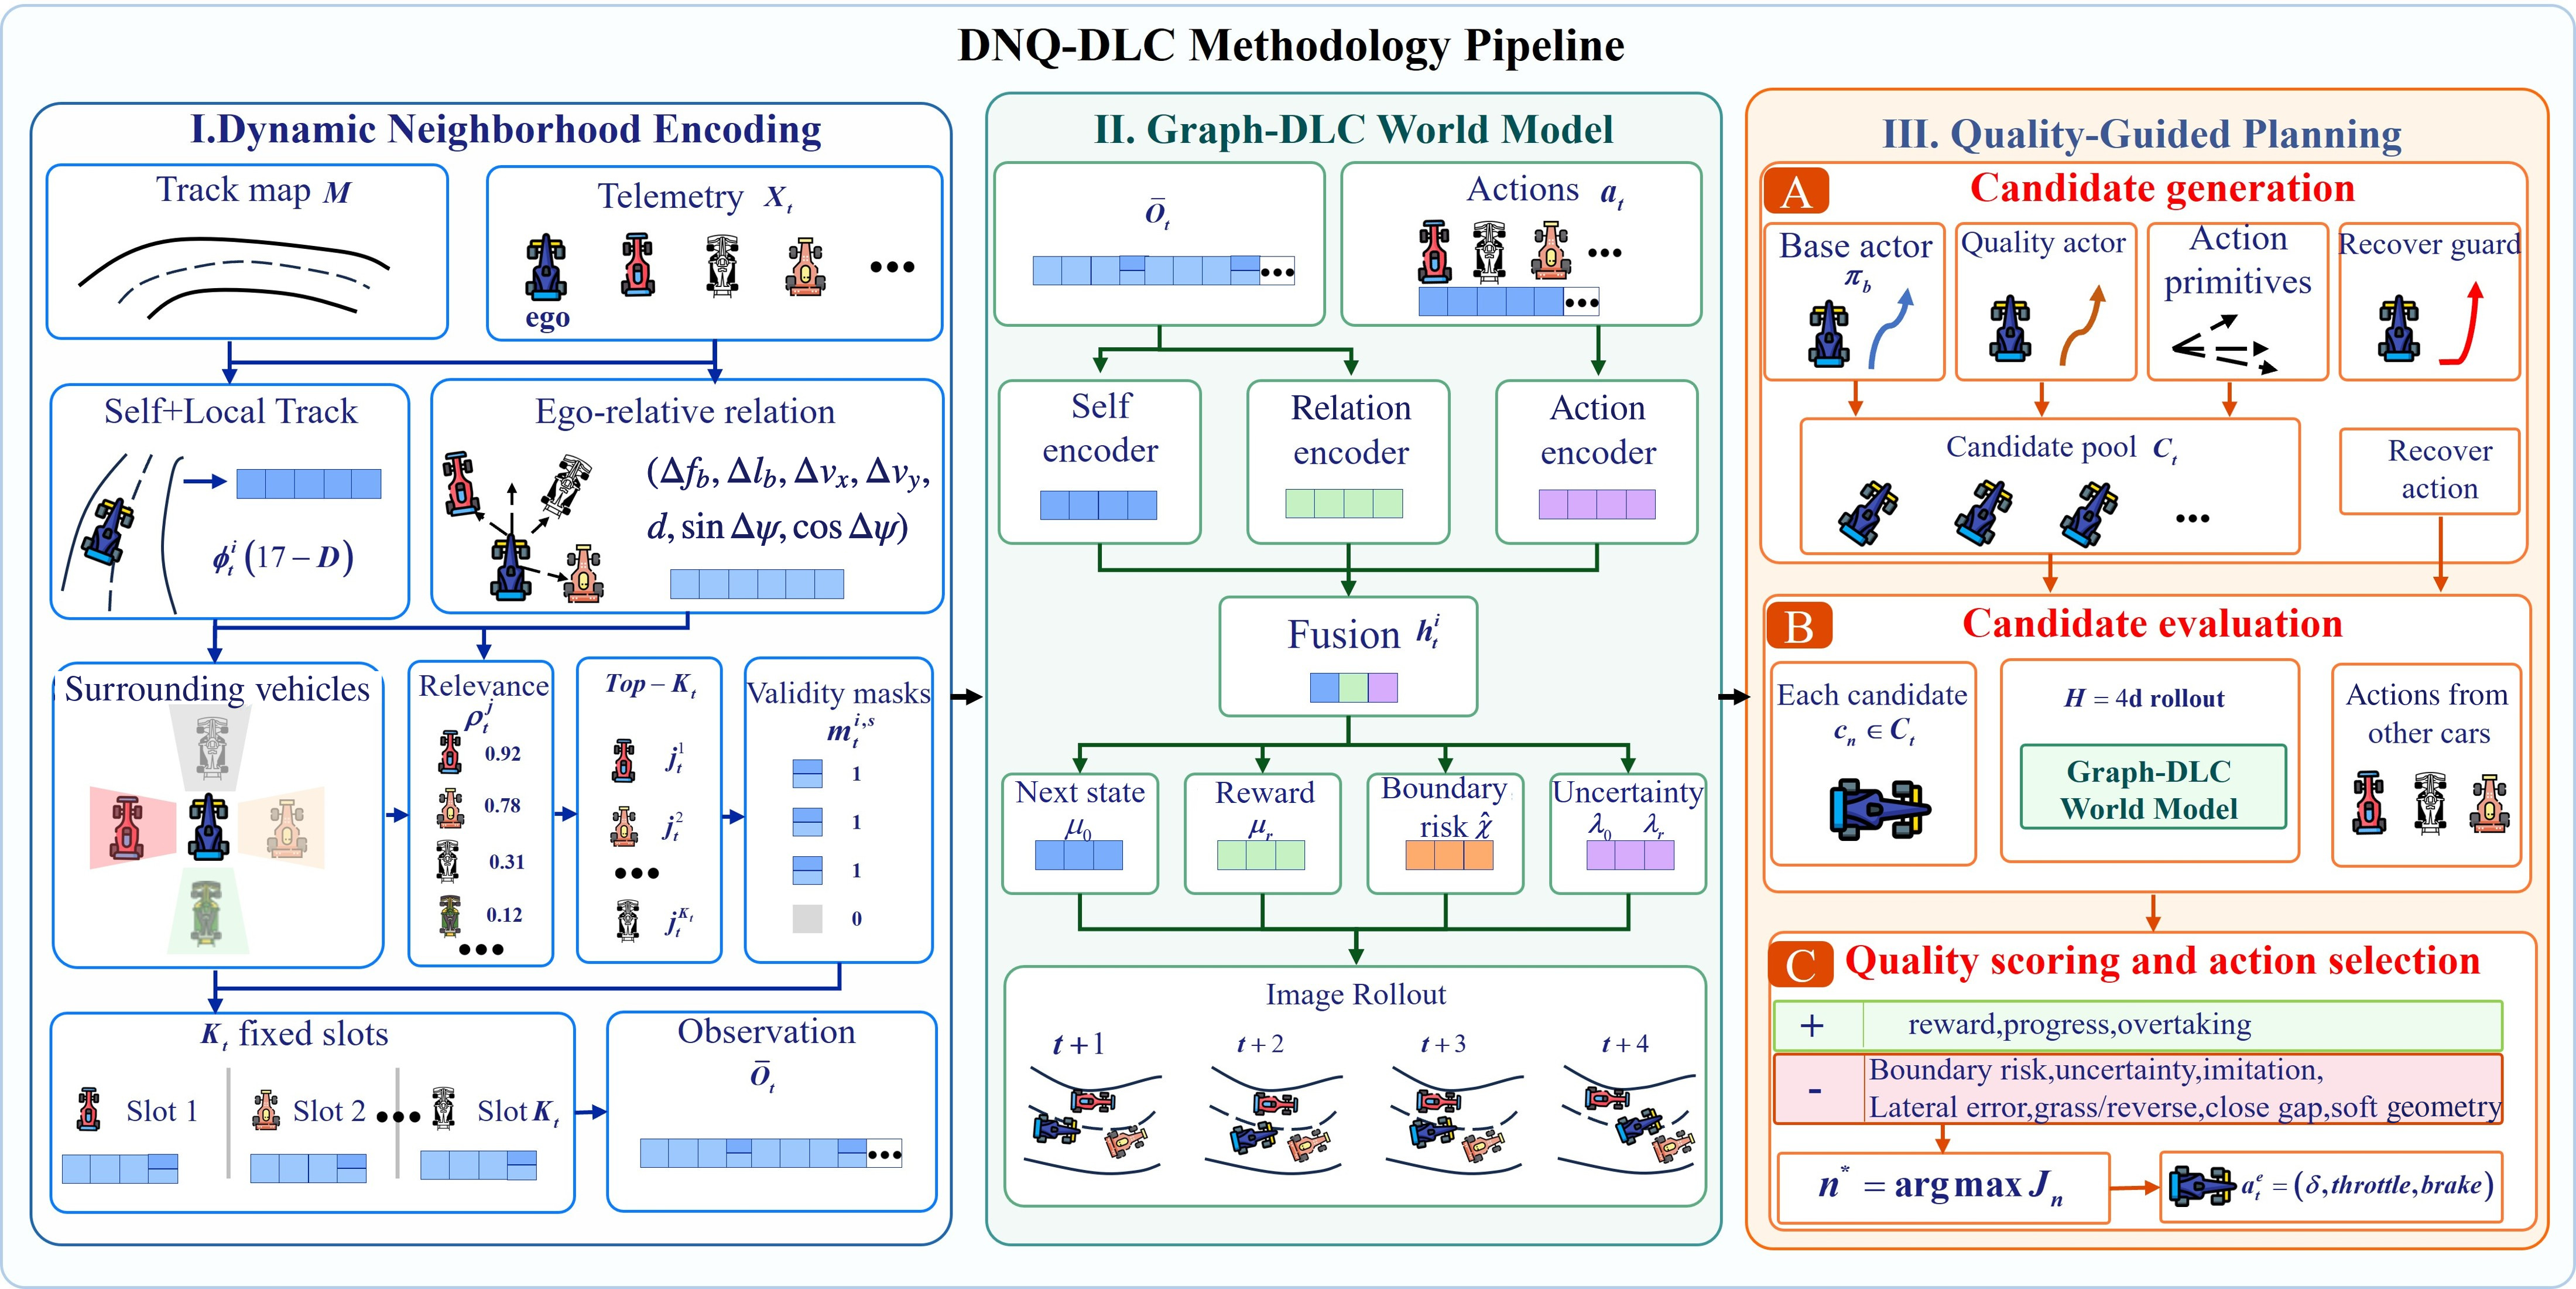
\includegraphics[width=0.86\textwidth]{figures/lct_9.16.jpg}
\caption{Overview of DNQ-DLC. Stage~I selects the dynamic
neighbourhood and packs the retained relations into masked slots $K_t$;
Stage~II predicts the next state, reward, boundary-risk proxy and log-variance
of each candidate action; Stage~III scores the imagined rollouts and commits the
first action of the best candidate unless the recovery guard fires.}
\label{fig:method_overview}
\end{figure*}

\subsection{Problem Formulation and Closed-Loop Framework}
\label{subsec:closed_loop}

Fig.~\ref{fig:method_overview} organizes the controller into three stages,
executed once per real decision step. The first encodes the dynamic
neighbourhood: the ego-relative relations of the exposed vehicles are ranked and
the retained ones packed into fixed slots with validity masks
(Section~\ref{subsec:graph_world_model}). The second predicts the next state,
reward, boundary-risk proxy and log-variance over the imagined horizon from the
self, relation and action encoders (Section~\ref{subsec:world_model}). The third
rolls a candidate pool through that same model, scores the rollouts and commits
the first action of the best candidate (Section~\ref{subsec:planning}). The
figure labels the slot block by a single count because the three capacities
coincide at the submitted operating point.

Let $\mathcal M$ denote the track map and let
$X_t=[x_t^i]_{i=1}^{N}$ be the joint telemetry at physical time $t$. The
controlled vehicle is indexed by $e$; all other rows are background vehicles.
The normalized control action is
\begin{equation}
 a_t^e=[\delta_t,u_t,b_t]^\top\in\mathcal A,
\end{equation}
where steering, throttle and braking are bounded by the simulator action
space. The planner maintains a candidate set $\mathcal C_t$ and an imagined
horizon $H$. For candidate $n$, $J_n$ denotes the discounted predicted
quality of its continuation. The receding-horizon decision is
\begin{equation}
 n^\star=\arg\max_{1\le n\le|\mathcal C_t|}J_n,\qquad
 a_t^e= a_t^{(n^\star),e}.
\label{eq:main_action_selection}
\end{equation}
Only $a_t^e$ is committed to the simulator. The next telemetry $X_{t+1}$
starts a new selection--packing--prediction cycle, so an imagined prediction
never changes the physical graph by itself.

\subsection{Dynamic Ego-Centric Interaction Graph}
\label{subsec:graph_world_model}

For each vehicle $j$ exposed by the runtime telemetry builder as a candidate
relation, the extractor forms an ego-relative relation
\begin{equation}
 r_t^{ej}=\left[\begin{array}{c}
 \Delta f_{b,t}^{ej},\Delta l_{b,t}^{ej},\Delta v_{x,t}^{ej},\Delta v_{y,t}^{ej},\ d_t^{ej},\\
 \sin\Delta\psi_t^{ej},\cos\Delta\psi_t^{ej}
 \end{array}\right]^\top\in\mathbb R^{d_r},
\label{eq:relation_vector}
\end{equation}
where $\Delta f_b$ and $\Delta l_b$ are displacements in the heading-defined
telemetry frame,
$\Delta v_x$ and $\Delta v_y$ are global-frame relative velocity components,
$d$ is separation, and $\Delta\psi$ is heading difference. Displacements and
distance are divided by the simulator spatial scale; velocities are divided
by its speed scale before encoding. The relation channels follow the
simulator's physical forward and left vehicle axes, so $\Delta l_b$ is a true
cross-track offset and $\Delta\psi$ the heading error against the local track
tangent. The channels are read in those vehicle axes rather than projected onto
the tangent, which would not measure a cross-track distance.

Let $\mathcal V_t^{\mathrm{cand}}$ denote the bounded candidate set exposed by
the telemetry builder at the current physical step. A candidate is eligible
if it lies inside radius $R_{\rm loc}$ or satisfies a forward, alongside, or
rear-pressure gate. With gate indicators $I_f,I_s,I_r$, this gives
\begin{equation}
\mathcal N_t=\{j\in\mathcal V_t^{\rm cand}:d_t^{ej}\le R_{\rm loc}
\ \vee\ I_f^j\vee I_s^j\vee I_r^j\}.
\end{equation}
All quantities in the gate and score are converted back to metric units.
For each eligible vehicle the selector computes
\begin{equation}
 \begin{aligned}
 \rho_t^j={}&w_f G_f(x_t^e,x_t^j)+w_s G_s(x_t^e,x_t^j)\\
 &+w_r G_r(x_t^e,x_t^j)+w_d q_d+w_{v,\rho}q_v\\
 &+w_{\psi,\rho}q_\psi-w_{d,\rho}d_t^{ej},
 \end{aligned}
\label{eq:relevance_score}
\end{equation}
where $I_f$ tests $0<\Delta f_b<f_f$, $|\Delta l_b|<l_f$;
$I_s$ tests $|\Delta f_b|<f_s$, $|\Delta l_b|<l_s$; and $I_r$ tests
$-f_r<\Delta f_b\le0$, $|\Delta l_b|<l_r$, $q_v>v_r$.
The continuous factors are
\begin{equation}
\begin{aligned}
G_f&=I_f[1-|\Delta f_b-f_0|/f_w]_+,\\
G_s&=I_s[1-|\Delta l_b|/l_s]_+,\qquad G_r=I_r,\\
q_d&=1/\max(d/d_0,1),\\
q_\psi&=[\cos\Delta\psi]_+-c_h|\sin\Delta\psi|.
\end{aligned}
\end{equation}
Here $[z]_+=\max(z,0)$, and $q_v$ is the closing speed obtained by projecting
the global-frame relative velocity on the controlled vehicle's own heading axis,
so it does not depend on the orientation of the world axes. Numerical
thresholds and weights of (\ref{eq:relevance_score}) are collected in
Table~\ref{tab:frozen_config}. The runtime sorts the
represented neighbours and returns an ordered, capacity-limited list
\begin{equation}
\begin{aligned}
 (j_t^1,\ldots,j_t^{K_t})&=\operatorname{Select}_{K_{\mathrm{cap}}}(\mathcal N_t;\rho_t),\\
 \widetilde{\mathcal N}_t&=\{j_t^s\}_{s=1}^{K_t},\qquad
 K_t=|\widetilde{\mathcal N}_t|\le K_{\mathrm{cap}}.
\end{aligned}
\label{eq:dynamic_selection}
\end{equation}
The list order is the slot order: for the controlled row $e$, the represented
neighbour $j_t^s$ occupies relation slot $s$. Both $\mathcal N_t$ and this
slot correspondence can change at every real decision time. $K_{\mathrm{cap}}$
is a computational capacity, not a fixed physical neighbourhood. We use
$K_{\mathrm{model}}$ for the fixed relation-slot width expected by the trained
checkpoint and decoder; it may be smaller than the runtime capacity after
repacking.

Each selected relation is paired with a validity indicator $m_t^{i,s}\in\{0,1\}$.
Because the learned checkpoint has a fixed interface, only the first
$\widetilde K_t=\min(K_t,K_{\mathrm{model}})$ selected relations are packed
into that interface. For the controlled row, model slot $s$ contains
$(r_t^{e j_t^s},1)$ when $s\le\widetilde K_t$ and a masked fill slot
otherwise. The remaining ranked relations are retained only in the runtime
selection record and cannot enter the fixed-width decoder tensor.
The same construction applies to other model rows when their local relations
are represented. The resulting slot vector is
\begin{equation}
 y_t^{i,s}=\bigl[r_t^{i,s},m_t^{i,s}\bigr]^\top\in\mathbb R^{d_y},\qquad d_y=d_r+d_m,\quad d_m=1,
\label{eq:relation_slot}
\end{equation}
with $m=0$ for padded slots; the mask suppresses their physical fill values. The packed
row observation is
\begin{equation}
\begin{aligned}
\bar o_t^i&=\bigl[\phi_t^i,y_t^{i,1},\ldots,y_t^{i,K_{\mathrm{model}}}\bigr]^\top\in\mathbb R^{d_o},\\
d_o&=d_\phi+K_{\mathrm{model}}d_y.
\end{aligned}
\label{eq:packed_observation}
\end{equation}
where $\phi_t^i$ contains the self state and local track descriptors. Three
distinct quantities are therefore involved and are kept apart throughout:
$K_{\mathrm{cap}}$ is the runtime capacity at which
opponents are ranked, $K_t$ is how many real relations were selected at this
step, and $K_{\mathrm{model}}$ is the width the checkpoint was trained with.
The graph is an ego-centred star. Selected vehicles are nodes, their
ego-relative features are the incident edges, and the learned interaction
operator is a masked mean over those edges.

\subsection{Action-Conditioned Graph World Model}
\label{subsec:world_model}

For agent row $i$, self, relation and action encoders are
\begin{equation}
 e_s^i=f_s(\phi_t^i),\qquad e_r^{i,s}=f_r(r_t^{i,s}),\qquad e_a^i=f_a(a_t^i).
\end{equation}
Masked aggregation prevents padded relations from contributing:
\begin{equation}
 e_r^i=\frac{\sum_{s=1}^{K_{\mathrm{model}}}m_t^{i,s}e_r^{i,s}}{\max(\sum_{s=1}^{K_{\mathrm{model}}}m_t^{i,s},1)}.
\label{eq:masked_aggregation}
\end{equation}
The local and scene-level summaries are fused as
\begin{equation}
\begin{gathered}
 h_t^i=f_h\bigl[e_s^i,e_r^i,e_a^i,\bar e_s,\bar e_a\bigr],\\
 \bar e_s=\operatorname{mean}_i e_s^i,\quad \bar e_a=\operatorname{mean}_i e_a^i.
\end{gathered}
\end{equation}
The transition heads output the next packed observation, reward, boundary-risk
logit and log-variance outputs:
\begin{equation}
\begin{gathered}
 (\mu_{t+1|t}^{o,i},\lambda_{t+1|t}^{o,i},\mu_{t+1|t}^{r,i},\lambda_{t+1|t}^{r,i},z_{t+1|t}^{\chi,i})=F(h_t^i),\\
 \hat\chi_{t+1|t}^i=\sigma(z_{t+1|t}^{\chi,i}).
\end{gathered}
\label{eq:transition_heads}
\end{equation}
The planner uses the model's predicted means. Training minimizes the
weighted point-prediction objective
\begin{equation}
\begin{aligned}
 \mathcal L_o&=\operatorname{MSE}(\mu^{o}_{t+1|t},\bar O_{t+1}),\\
 \mathcal L_r&=\operatorname{MSE}(\mu^{r}_{t+1|t},r_{t+1}),\\
 \mathcal L_\chi&=\operatorname{BCEWithLogits}(z_{t+1|t}^{\chi},\chi_{t+1}),\\
 \mathcal L_{\rm prop}&=\mathbb E_i\operatorname{MSE}(\pi_b(\bar o_t^i),a_t^i),\\
 \mathcal L&=\mathcal L_o+\alpha_r\mathcal L_r+\alpha_\chi\mathcal L_\chi\\
 &\quad+\alpha_p\mathcal L_{\rm prop}+\lambda_q\mathcal L_q
 +\mathcal L_v,
 \\[-1mm]
 &\qquad \mathcal L_v=0.01\left(|\mathbb E\lambda^o|+|\mathbb E\lambda^r|\right).
\end{aligned}
\label{eq:training_objective}
\end{equation}
Here $\pi_b$ is the base actor and $\mathcal L_q$ is an optional auxiliary
quality-head loss. In the submitted configuration $\lambda_q=0$; quality
guidance is supplied by a separately behaviour-cloned quality actor $\pi_q$,
not by an active auxiliary prediction head. MSE averages squared scalar
errors over samples and output entries; base-actor supervision includes all
vehicle rows. BCE and variance expectations use mean reductions over the
batch and represented rows. Here $r_{t+1}$ is the reward returned after
executing $a_t$. In the rollout equations below, $\hat r_{t+\tau}^{(n)}$
denotes the predicted reward for the transition from $t+\tau$ to
$t+\tau+1$, indexed by its starting time; at $\tau=0$ it is the ego-row
reward mean $\mu_{t+1|t}^{r,e}$.
The variance outputs receive this regularizer but no likelihood-based
calibration loss, so $C_u$ is a proxy for how far the imagined transition sits
from the fitted mean, not a calibrated predictive variance, and it is used at
the small weight the table gives it: over $7{,}920$ transitions sampled from the
released collection episodes the two predicted log-variances sum to a channel
with standard deviation $0.04$ that never leaves $[-0.5,0.5]$, so its
contribution to $J_n$ is about four per cent of the risk term's. The risk target
is a telemetry flag for grass, backward motion, or excessive absolute lateral
telemetry; it does not estimate collision probability.

The world model and base actor use 160 collection episodes with 352,000
transitions from expert telemetry policies and 4--6 vehicles. In every episode
the recorded vehicle is driven by the joint-clearance pilot and the remaining vehicles
hold a constant 13~m/s lane target. Adam training
runs for 40{,}000 updates of batch size 512 with a learning rate decaying from
$3\times10^{-4}$ on a cosine schedule.
The quality actor minimizes
$\mathcal L_{\rm BC}=\mathbb E_{(o,a)\sim\mathcal D_q}\operatorname{MSE}(\pi_q(o),a)$
on 1,526 accepted on-track event samples from 24 separate collection
episodes. Failed events are excluded from $\mathcal D_q$; this is a
conditional imitation prior, not learned evidence of safe behaviour in failure
states. Episode-disjoint predictive validation is performed after freezing the
checkpoint and is not used for model selection: the submitted transition model is
the endpoint of the fixed $40{,}000$-update cosine schedule, so no validation
quantity was consulted before that endpoint was fixed. Section~\ref{sec:experiments}
reports the realized error of that imagined rollout.

\paragraph{Fusing the draws}
The recipe above is stochastic, and Section~\ref{sec:experiments} reports five
draws of it whose strict-tier counts span fourteen to twenty-six of the
forty-eight cases; the submitted controller is the first of them. Because
retraining the transition model moves the endpoint counts by more than the gaps
between the controllers compared below, Section~\ref{sec:experiments} reports
every learned method as the mean over the draws of its recipe rather than as a
single checkpoint, and the fused variant defined below is released as an
alternative to the submitted controller. The transition model of
\eqref{eq:transition_heads} is trained $M=5$ times on the same data under the
same schedule, and the planner consumes the fused heads
\begin{equation}
\begin{gathered}
 \bar\mu^{o}_{t+1|t}=\frac{1}{M}\sum_{j=1}^{M}\mu^{o,(j)}_{t+1|t},\\
 \bar\lambda^{o}_{t+1|t}=\log\Bigl(\frac{1}{M}\sum_{j=1}^{M}
 e^{\lambda^{o,(j)}_{t+1|t}}
 +\operatorname{Var}_{j}\bigl[\mu^{o,(j)}_{t+1|t}\bigr]\Bigr),
\end{gathered}
\label{eq:member_fusion}
\end{equation}
where the superscript $(j)$ indexes the member. The first term inside the
logarithm is the aleatoric variance the members report between them, and the
second is their disagreement, which no member can see on its own
~\cite{lakshminarayanan2017simple,chua2018pets}.
Equation~\eqref{eq:planner_costs} reads the uncertainty cost off the same
log-variance, so a candidate whose outcome the members disagree about is
penalized in proportion to that disagreement. Reward, risk logit and the
auxiliary quality head are averaged in the same way. The proposal actor, the
quality actor and the planner constants are not fused: they are single
instances shared by the members, so \eqref{eq:member_fusion} is the only
difference between the fused variant and the controller of
Table~\ref{tab:main_comparison}.
Fusion multiplies the cost of one imagined rollout by $M$ and raises the mean
decision time from 243~ms to 443~ms over the 48 cases; it is released with the
controller and is not the reported result. No evaluation case
was used to select the members or to weight them. Both are wall-clock means,
read against the control interval: the simulator advances $0.02$~s per step, so
the four-step ranking spans $0.08$~s while one decision costs 243~ms. Neither the
single model nor the fused policy ranks inside one control interval on the
evaluation machine, and the evaluation applies each decision at the next step
without simulating that delay, which is itself a control problem in
racing~\cite{kalaria2024delay}, so the endpoints below describe the algorithm
rather than a real-time control loop. Closing the gap would take a smaller
candidate budget, a shorter horizon or a batched rollout; the fused policy would
also need fewer members.

\subsection{Quality-Guided Predictive Planning}
\label{subsec:planning}

The candidate set combines learned proposals and interpretable action
primitives:
\begin{equation}
\begin{gathered}
 \mathcal U_t=\left\{\begin{array}{l}
 \pi_b(\bar o_t^e),\pi_q(\bar o_t^e),c_{\rm chase},c_{\rm anchor},\\
 c_{\rm pass},c_{\rm brake},c_{\rm rec},c_{\rm ret},c_{\rm pert}
 \end{array}\right\},\\
 \mathcal C_t=\operatorname{Unique}_B(\mathcal U_t).
\end{gathered}
\label{eq:candidate_pool}
\end{equation}
$\operatorname{Unique}_B$ removes duplicate normalized actions and retains
at most the configured candidate budget $B$. In the pool, $\pi_b$ and $\pi_q$
are the learned proposal and quality actors; $c_{\rm anchor}$ is the command of
a rule-based telemetry expert gate of the same family as the rule-expert
reference; $c_{\rm chase}$ closes up on the vehicle ahead; $c_{\rm pass}$ and
$c_{\rm brake}$ are the lane-change and braking manoeuvres; $c_{\rm rec}$ and
$c_{\rm ret}$ are the recovery action and its graded corridor-return variants,
both defined below; and $c_{\rm pert}$ is a fixed perturbation profile around
the proposal. Templates are enabled by their corresponding telemetry gates, and
their constants belong to the released planner code.

A feasibility guard handles states in which ordinary overtaking candidates
would be extrapolated outside the training support. Let $\zeta_t$ indicate
backward motion, severe track departure, or an unsafe heading. While it fires,
the guard's recovery command is one candidate among the others; the committed
action is
\begin{equation}
 \begin{aligned}
 \mathcal E_t&=\begin{cases}
 \{n:\phi^{(n)}=0\},&\zeta_t^{\rm esc}=1,\\
 \{1,\ldots,|\mathcal C_t|\},&\text{otherwise},
 \end{cases}\\
 a_t^e&=\begin{cases}
 a_t^{\rm rec},&\zeta_t^{\rm esc}=1\ \text{and}\ \mathcal E_t=\varnothing,\\
 a_t^{(n^\star),e},&\text{otherwise},\quad n^\star=\arg\max_{n\in\mathcal E_t}\tilde J_n,
 \end{cases}
 \end{aligned}
\label{eq:recovery_guard}
\end{equation}
where $\mathcal E_t$ is the eligible set and $\tilde J_n$ is the constrained
score defined below.
Here $a_t^{\rm rec}$ is the corridor-return action the reported runs execute.
Its steering component is a bounded cross-track return law,
\begin{equation}
 a_t^{\rm rec,s}=\operatorname{clip}\!\left(g_r\varsigma_t-g_\psi\Delta\psi_t,-1,1\right),
\label{eq:return_law}
\end{equation}
where $\varsigma_t$ is the signed cross-track channel of the corrected
telemetry, $\Delta\psi_t$ is the heading error to the local track tangent in
radians, and the two gains are $g_r=1.4$ and $g_\psi=1.6$. The sign of
$\varsigma_t$ is fixed by the vehicle's own lateral response, measured once in
the simulator, not read off the protocol: a vehicle placed off the centreline
returns with $\operatorname{sgn}(a_t^{\rm rec,s})=\operatorname{sgn}(\varsigma_t)$
and diverges with the opposite sign. Throttle is
$0.55$ below a $17.5$~m/s reference that is reduced by the corner and lateral
errors and floored at $12$~m/s, and $0.08$ above it, with braking applied
$3$~m/s above that reference. The command passes through
the same speed and geometry limiter as the candidate actions, so it respects the
same vehicle limits as everything else, and the candidate pool additionally
carries the archived rule-recovery template when the real state is infeasible.
This guard is enabled for the reported DNQ-DLC runs. It is a feasibility
fallback rather than a learned policy. The escalation indicator
$\zeta_t^{\rm esc}$ is defined with the state-feasibility violation below, and
the escalation window and the guard thresholds appear in
Table~\ref{tab:frozen_config}.

Equation~\eqref{eq:return_law} replaces the archived track-follower, which aimed
at the centreline eight tiles ahead and folded the offset into a heading command,
$1.05\,\ell/40$, wrapped to $(-\pi,\pi]$. At that gain the lateral term reaches
the steering lock only beyond about $25$~m of offset, while the runs contain
vehicles $10$ to $17$~m off the centreline that took hundreds of steps to return
or never returned. Raising the gain is not a repair, because the wrap then enters
the operating range: at a gain of $8$ a $17$~m offset inverts the command and
drives the vehicle outward. Three properties of the return layer follow from
the same measurement. It is gated at $0.90$ half-widths so a pass keeps its full
lateral envelope inside that offset. It defers while a vehicle is alongside and
the ego is still inside the road edge, because cutting back to the racing line
with a car in the adjacent lane is a contact rather than a recovery; outside the
road edge it acts unconditionally. When it acts, its graded variants
$c_{\rm ret}$ are inserted at the head of $\mathcal C_t$ and it also overrides
the steering component of $a_t^{\rm rec}$.
The layer was fixed before the 48-case evaluation was re-run, and its effect was
checked on six dense-field episodes outside those 48 cases (seeds 33 to 38 at
six vehicles, under the submitted world-model draw): the strict tier rises from
two to three of the six, the in-corridor share of the manoeuvre window from
0.88 to 0.98, and the whole-episode grass fraction falls from 0.112 to 0.064, at
a completion of six either way. Six episodes are too few to separate the two
layers, so that check is reported as a direction rather than as an effect.

For each candidate, the first target action is fixed to the candidate and
later target actions follow a quality-guided continuation
\begin{equation}
\begin{aligned}
 a_t^{(n),e}&=c_n,\\
 \tilde a_{t+\tau}^{(n),e}&=(1-\alpha_q)\pi_b(\hat{\bar o}_{t+\tau|t}^{e,(n)})\\
 &\quad+\alpha_q\pi_q(\hat{\bar o}_{t+\tau|t}^{e,(n)}),\\
 a_{t+\tau}^{(n),e}&=\mathcal S_t(\tilde a_{t+\tau}^{(n),e},
 \hat{\bar o}_{t+\tau|t}^{e,(n)}),\quad\tau>0.
\end{aligned}
\label{eq:actor_continuation}
\end{equation}
Here $\mathcal S_t$ is the deterministic speed/geometry limiter also applied
before candidate deduplication: it caps throttle, increases braking, and
attenuates steering when speed or geometry thresholds are exceeded.
The quality policy includes its own relation repacking before inference.
Non-target actions are generated by the configured background-policy set
$\Pi_{\rm bg}$. Let $\mathcal F$ denote the complete encoder--transition--decoder
map whose output heads are $F$ in (\ref{eq:transition_heads}). It is iterated as
\begin{equation}
\begin{gathered}
 \bigl(\hat{\bar O}_{t+\tau+1|t}^{(n)},\hat r_{t+\tau}^{(n)},\hat\chi_{t+\tau+1|t}^{(n)}\bigr)
 =\mathcal F\bigl(\hat{\bar O}_{t+\tau|t}^{(n)},a_{t+\tau}^{(n)}\bigr),\\
 \hat{\bar O}_{t|t}^{(n)}=\bar O_t.
\end{gathered}
\label{eq:rollout_recurrence}
\end{equation}
The transition tensor preserves slot positions and validity masks throughout
the imagined horizon. The quality-actor input is repacked from the predicted
relations at each continuation step, which can reorder the represented slots
but cannot introduce an unobserved vehicle; only the next real observation
refreshes the physical candidate set. Because the selector re-ranks at every
real step, a fixed slot position does not by itself guarantee that a decoder
channel tracks the same physical vehicle across a rank change. Within one
decision the correspondence is consistent, which is what the candidate scores
rely on; across decisions the graphs are rebuilt from telemetry rather than
carried over.

The candidate score is
\begin{equation}
\begin{aligned}
 J_n=\sum_{\tau=0}^{H-1}\gamma^\tau\Big[&\hat r_{t+\tau}^{(n)}+\lambda_pR_p^{(n,\tau)}+\lambda_oR_o^{(n,\tau)}\\
 &-\lambda_\chi C_\chi^{(n,\tau)}-\lambda_u C_u^{(n,\tau)}-\lambda_{\rm live}C_{\rm live}^{(n,\tau)}\\
 &-\lambda_i C_i^{(n,\tau)}-\lambda_\ell C_\ell^{(n,\tau)}-\lambda_g C_g^{(n,\tau)}\\
 &-\lambda_c C_c^{(n,\tau)}-\lambda_f C_f^{(n,\tau)}\\
 &+\lambda_r R_r^{(n,\tau)}\Big].
 \end{aligned}
\label{eq:planner_score}
\end{equation}
The progress, risk and stall terms are
\begin{equation}
\begin{aligned}
 R_p^{(n,\tau)}&=\hat\eta_{t+\tau+1|t}^{(n)}-\hat\eta_{t+\tau|t}^{(n)},\qquad
 C_\chi^{(n,\tau)}=\hat\chi_{t+\tau+1|t}^{(n)},\\
 C_{\rm live}^{(n,\tau)}&=[v_{\rm live}-\hat v_{t+\tau+1|t}^{(n)}]_+/v_{\rm live},
\end{aligned}
\end{equation}
\begin{equation}
\begin{aligned}
R_o^{(n,\tau)}={}&w_\mathrm{pass}\,|\{j\in\mathcal A^\tau:\tilde\lambda_j^{\tau+1}\le-\ell_{\rm clr}\}|\\
 &+\mathbb I[\mathcal A^\tau\neq\varnothing,\mathcal A^{\tau+1}\neq\varnothing]\\
 &\quad\times\operatorname{clip}\left(\frac{\min_j\tilde\lambda_j^{\tau}-\min_j\tilde\lambda_j^{\tau+1}}{L_g},-r_-,r_+\right)\\
 &+w_a[|\mathcal A^\tau|-|\mathcal A^{\tau+1}|]_++w_v[v_{t+\tau+1}-v_c]_+.
\end{aligned}
\label{eq:overtaking_reward}
\end{equation}
Here $\eta$ is normalized visited-track progress, $v_{\rm live}$ is the pace
below which a rollout is priced as stalled, and
\begin{equation}
\begin{aligned}
 \tilde\lambda_j&=\rho_j^{\parallel}\cos e_\psi+\rho_j^{\perp}\sin e_\psi,\qquad
 \check\lambda_j=\rho_j^{\parallel}\sin e_\psi-\rho_j^{\perp}\cos e_\psi,\\
 \mathcal A^\tau&=\bigl\{j:0<\tilde\lambda_j^\tau<L_c,\ |\check\lambda_j^\tau|<L_\perp\bigr\}.
\end{aligned}
\label{eq:track_frame_lead}
\end{equation}
$\rho_j^{\parallel},\rho_j^{\perp}$ are the packed body-frame slot relations
of neighbour $j$ and $e_\psi$ is the target's own heading error, so
(\ref{eq:track_frame_lead}) is the same relation expressed in the frame of the
local track tangent; $\mathcal A^\tau$ is the set of vehicles still ahead of the
ego inside the approach cone and $|\mathcal A^\tau|$ is $n_{\rm ahead}$.
The cone has length $L_c$ and lateral half-width $L_\perp$, both in metres;
$L_\perp$ is wider than the simulated road, so the cone acts as a longitudinal
gate rather than a lateral one. $L_g$ appears only in the denominator of the
graded term of (\ref{eq:overtaking_reward}) and is the length that maps a lead
change onto the clip $[-r_-,r_+]$; it is set equal to $L_c$, so closing one cone
length saturates the grading.
The same quantity enters the overtaking credit: an opponent counts as cleared
in (\ref{eq:overtaking_reward}) once its track-frame lead $\tilde\lambda_j$
passes $-\ell_{\rm clr}$, and the lead change over one step is measured as the
change in the smallest $\tilde\lambda_j$ over the approach cone. The numerical
values of $w_{\rm pass}$, $\ell_{\rm clr}$, $L_g$, $r_\pm$, $w_a$, $w_v$ and
$v_c$ are in Table~\ref{tab:frozen_config}.
The frame matters because a body-frame cone can be left by yaw alone: with the
body-frame version of this term, a candidate that steered hard pushed the
leading vehicle out of the cone and collected the full clearance credit without
changing the along-track order, so the planner could hold a hard steering
angle while the order ahead stayed the same. The
track-frame lead $\tilde\lambda_j$ in (\ref{eq:track_frame_lead}) changes only
when the along-track order changes, so the credit has to be earned by closing
up or by passing. The overtaking reward is replaced by $\min(R_o,0)$ when the
predicted target is on grass, moves backward, or satisfies
$|\hat\ell|>\ell_g$.
The remaining costs use the predicted target's lateral telemetry $\hat\ell$
and heading deviation $e_\psi=\arccos(\operatorname{clip}(c_\psi,-1,1))$.
The proposal set is $\Pi=\{\pi_b,\pi_q\}$, with
$\tilde a_{\pi,t}=\pi(\bar o_t^e)$. These imitation references are held at
their real-step values even though continuation actions are recomputed.
\begin{equation}
\begin{aligned}
 C_\ell&=|\hat\ell|+w_\psi|e_\psi|+w_{\ell,e}[|\hat\ell|-\ell_e]_+\\
 &\quad+w_{\psi,e}[c_{\psi,\min}-\cos(e_\psi)]_+,\\
 C_g&=w_{\rm grass}\mathbb I[\mathrm{grass}]+w_{\rm back}\mathbb I[\mathrm{back}]\\
 &\quad+w_{\ell,g}[|\hat\ell|-\ell_g]_+,\\
 C_c&=[g_c-d_{\mathrm{front}}]_+/g_c,\\
 C_u&=\operatorname{clip}(\lambda^o+\lambda^r,u_-,u_+),\\
 d_{\pi}^{(n,\tau)}&=\frac{1}{d_a}\left\lVert a_{t+\tau}^{(n),e}
 -\tilde a_{\pi,t}\right\rVert_2^2,\\
 C_i&=\min_{\pi\in\Pi}d_{\pi}^{(n,\tau)}.
 \end{aligned}
\label{eq:planner_costs}
\end{equation}
The corridor-return credit in \eqref{eq:planner_score} is
\begin{equation}
 R_r^{(n,\tau)}=\mathbb I[\tau=0]\,\mathbb I[\rho_t]\,\hat\kappa_t\,c_{n,\rm s},
 \qquad \hat\kappa_t=\operatorname{clip}(g_r\varsigma_t,-1,1),
 \label{eq:return_credit}
\end{equation}
where $c_{n,\rm s}$ is the steering component of candidate $n$ and $\rho_t$
is the gate of the return layer defined above: the credit is paid once, at the
real decision step, and only when the layer may act. It is deliberately
model-free. Over a four-step horizon the learned rollout is smooth in its
cross-track channel, so candidates whose steering commands point in opposite
directions differ by much less in predicted offset than they do in realized
offset, and \eqref{eq:planner_score} cannot separate a returning command from a
lane-keeping one on that channel alone; scoring the command against the measured
offset puts the direction back into the ordering. The gap is quantified on the
audited draws in Section~\ref{sec:mechanism_evidence}. The credit is inactive inside the
gate, so it does not bias an ordinary pass, and it is the only term in
\eqref{eq:planner_score} that is not read from the world model.
The active feasibility cost is a soft geometry-dependent penalty:
\begin{equation}
\begin{aligned}
 C_f={}&\lambda_{\rm geom}\Big\{
 \kappa[v-v_{{\rm ref},t}]_+/v_g\\
 &+[|\hat\ell|-\ell_f]_+(1+\beta_\ell\kappa)\\
 &+[c_f-\cos(e_\psi)]_+(1+\beta_\psi\kappa)\\
 &+\beta_g\mathbb I[\mathrm{grass}](1+\beta_\kappa\kappa)\Big\}.
\end{aligned}
\label{eq:feasibility_cost}
\end{equation}
Here $d_a$ is the action dimension; $\kappa$ is the absolute wrapped track-angle
change divided by the centreline-index lookahead span, not metric curvature.
It and the geometry-dependent target speed $v_{{\rm ref},t}$ are computed
at the real decision step and held fixed during the imagined horizon;
$v_g$ is the speed normalization for this penalty. The optional base penalty
is disabled in the submitted configuration. This cost is not a control barrier function and does not provide a formal collision
or safety guarantee. The quality actor is the active quality-guidance module,
and the auxiliary quality head in (\ref{eq:training_objective}) is an optional
training output that is inactive in the submitted checkpoint, where
$\lambda_q=0$.

\paragraph{State feasibility as a separate penalty}
Two closed-loop constraints are evaluated on the imagined states and
accumulated as one violation that is priced by $\lambda_\phi$ rather than
folded into the geometry penalty (\ref{eq:feasibility_cost}):
\begin{equation}
\begin{aligned}
\phi_g&=\mathbb I[\mathrm{back}]+\mathbb I[\mathrm{grass}]\bigl(1+[|\hat\ell|-\ell_{\rm guard,grass}]_+\bigr)\\
 &\quad+[|\hat\ell|-\ell_{\rm guard}]_+ +[c_{\rm guard}-\cos\hat e_\psi]_+,\\
\phi_c&=\sum_{j}\bigl[\ell_{\rm cl}-|\hat\rho_j^{\perp}|\bigr]_+
 \mathbb I\bigl[|\hat\rho_j^{\parallel}|\le\ell_{\rm ab}\bigr]m_j,\\
\phi^{(n,\tau)}&=\phi_g+\phi_c,
\end{aligned}
\label{eq:state_feasibility}
\end{equation}
so that $J_n$ in (\ref{eq:planner_score}) carries the extra term
$-\lambda_\phi\sum_{\tau=0}^{H-1}\gamma^\tau\phi^{(n,\tau)}$.
In (\ref{eq:state_feasibility}), $\phi_g$ is the guard severity (backward
motion, grass, roadside offset, heading), $\phi_c$ is the swept lateral-clearance
shortfall of every longitudinally overlapping neighbour, and $m_j$ is the slot
validity mask. $\ell_{\rm cl}$, $\ell_{\rm ab}$, $\ell_{\rm guard}$ and the
tighter grass threshold $\ell_{\rm guard,grass}$ are the clearance,
alongside-length and guard thresholds, all stated in
Table~\ref{tab:frozen_config} and expressed in road half-widths, the units of
the corrected lateral channel. The stall cost is deliberately not part of this
violation: it is the score term $C_{\rm live}$ of (\ref{eq:planner_score}),
priced at $\lambda_{\rm live}$, because the guard prices geometry while the
stall cost has to trade against progress inside the same sum.

The violation enters the objective as a soft penalty and also orders the pool.
Candidates are grouped by $\operatorname{round}(\phi^{(n)},10^{-2})$ and the
objective only breaks ties inside a group, that is
$\tilde J_n=J_n-\Lambda\operatorname{round}(\phi^{(n)},10^{-2})$ with $\Lambda$
larger than any objective difference the pool can produce, so the ranking is by
$(\phi,-J)$ with feasibility first, the usual order of constrained
model-predictive control. Pricing the violation is not by itself sufficient for
this pool: an earlier configuration that carried the soft penalty but ordered
by the objective alone left the corridor on 43\,\% of closed-loop steps, while
the imitation actor the planner blends towards held $|\hat\ell|\le0.95$ road
half-widths with no grass at all.

The guard is a filter, not a takeover: while $\zeta_t=1$ its recovery command is
one member of $\mathcal C_t$ and the remaining candidates are still scored, so
the planner keeps control of the committed action. A filter on its own has no
fallback, because once the vehicle already sits outside the guard band every
candidate inherits a positive violation at the first imagined step; in one
archived case the target stayed at $|\hat\ell|\approx5.3$ half-widths and
$0$~m/s for $2{,}000$ steps, every candidate that would have left the state
being scored on an out-of-distribution imagined state. The shield therefore
escalates
\begin{equation}
\zeta_t^{\rm esc}=\mathbb I\Bigl[\textstyle\sum_{s=t-N+1}^{t}\zeta_s\ge N\Bigr],
\label{eq:shield_escalation}
\end{equation}
after which the eligible set $\mathcal E_t$ of (\ref{eq:recovery_guard}) shrinks
to the candidates whose imagined rollout never enters the guarded state, and
only when that set is empty does the recovery command replace the committed
action. The streak counter $\sum_s\zeta_s$ resets on the first feasible real
state, so the escalation is a bounded-duration restriction tied to a measurable
condition on the real observations rather than a mode switch on a predicted
quantity.

Equations~(\ref{eq:dynamic_selection})--(\ref{eq:shield_escalation}) define the
individual operations. Algorithm~\ref{alg:dnqdlc} puts them in the order they
run at one physical decision time, and marks where graph refresh ends and
imagined propagation begins.

\begin{algorithm}[!b]
\caption{DNQ-DLC online decision at physical time $t$.}
\label{alg:dnqdlc}
\begin{minipage}{0.96\columnwidth}
\scriptsize
\noindent\rule{\linewidth}{0.45pt}\vspace{2pt}
\algreset
\State{\textbf{Input:} $X_t,\mathcal M,\mathcal F,\pi_b,\pi_q,\Pi_{\mathrm{bg}},\mathcal A$; $H,\gamma,N$; capacities $K_{\mathrm{cap}},K_{\mathrm{model}},B$}
\State{\textbf{Output:} committed target action $a_t^e$}
\noindent\rule{\linewidth}{0.35pt}\vspace{2pt}
\State{From the runtime-exposed candidate set in $X_t$, construct the gated relation set $\mathcal N_t$}
\State{For each $j\in\mathcal N_t$, compute its relevance score $\rho_t^j$ using (\ref{eq:relevance_score})}
\State{Order and retain represented neighbours $(j_t^1,\ldots,j_t^{K_t})$; define $\widetilde{\mathcal N}_t$ using (\ref{eq:dynamic_selection})}
\State{Retain the first $\min(K_t,K_{\mathrm{model}})$ relations; assign them to slots and mask unused slots}
\State{Pack $\bar O_t$ from the slot relations and masks using (\ref{eq:relation_slot})--(\ref{eq:packed_observation})}
\State{Update the feasibility streak and $\zeta_t^{\mathrm{esc}}$ using (\ref{eq:shield_escalation})}
\State{Generate $\mathcal C_t$ using (\ref{eq:candidate_pool}) and budget $B$, adding the recovery command when $\zeta_t=1$}
\State{\textbf{for each} $c_n\in\mathcal C_t$ \textbf{do}}
\StateCont{Initialize $\hat{\bar O}_{t|t}^{(n)}\gets\bar O_t$, fix $a_t^{(n),e}\gets c_n$, and set $J_n\gets0$}
\StateCont{\textbf{for} $\tau=0,\ldots,H-1$ \textbf{do}}
\StateInner{Generate background actions; use (\ref{eq:actor_continuation}) for target continuation}
\StateInner{Predict one step with (\ref{eq:rollout_recurrence}) using fixed transition-tensor slot positions}
\StateInner{Carry forward $m_t^{i,s}$; quality-actor repacking uses predicted relations only}
\StateInner{Accumulate the objective $J_n$ and the violation $\phi^{(n)}$ from (\ref{eq:planner_score})--(\ref{eq:feasibility_cost})}
\StateCont{\textbf{end for}}
\State{\textbf{end for}; order $\mathcal C_t$ by $(\phi,-J)$}
\State{\textbf{if} $\zeta_t^{\mathrm{esc}}=1$ \textbf{then} reduce $\mathcal C_t$ to the candidates with $\phi^{(n)}=0$ and commit $a_t^{\rm rec}$ if that set is empty}
\State{Commit $a_t^e\gets a_t^{(n^\star),e}$ from the leading candidate; execute it, observe $X_{t+1}$, and repeat from the new real observation}
\vspace{2pt}\noindent\rule{\linewidth}{0.45pt}
\end{minipage}
\end{algorithm}

The online loop is
$X_t\rightarrow\mathcal N_t\rightarrow\bar O_t\rightarrow\mathcal C_t$
$\rightarrow J_n\rightarrow a_t^e\rightarrow X_{t+1}$, in which
$\widetilde{\mathcal N}_t$ and its slot correspondence are updated at run time
while the packed interface keeps its width. The mechanism is evaluated as part
of the complete controller; a selector-only comparison is reported as a
diagnostic and does not by itself establish a general completion gain.

\begin{table*}[!t]
\centering
\caption{Frozen constants of the submitted controller:
selector, planner geometry and shield. Lengths are in metres, the gate and guard
distances in road half widths, and $c_f$, $c_{\mathrm{guard}}$,
$c_{\psi,\min}$ and $c_h$ are heading cosines.}
\label{tab:frozen_config}
\scriptsize
\setlength{\tabcolsep}{4pt}
\begin{tabular}{@{}lcc@{\hspace{16pt}}lcc@{}}
\toprule
Quantity & Symbol & Value & Quantity & Symbol & Value \\
\midrule
Rollout horizon & $H$ & 4 & Progress weight & $\lambda_p$ & 1.20 \\
Candidate budget & $B$ & 12 & Overtaking weight & $\lambda_o$ & 2.40 \\
Relation slots & $K_{\mathrm{model}}$ & 3 & Grass, lateral, close-gap & $\lambda_g$, $\lambda_\ell$, $\lambda_c$ & 2.00, 0.42, 0.65 \\
Runtime capacity & $K_{\mathrm{cap}}$ & 3 & Quality increments & $\Delta\lambda_o$, $\Delta\lambda_\ell$, $\Delta\lambda_g$, $\Delta\lambda_c$ & 0.60, 0.60, 1.00, 0.20 \\
Row, relation, packed dim. & $d_\phi$, $d_r$, $d_o$ & 17, 7, 41 & Risk, unc., live, guard & $\lambda_\chi$, $\lambda_u$, $\lambda_{\mathrm{live}}$, $\lambda_\phi$ & 1.65, 0.40, 1.50, 5.00 \\
World, actor width & $d_h$, $d_p$ & 192, 128 & Clearance, alongside, gate & $\ell_{\mathrm{cl}}$, $\ell_{\mathrm{ab}}$, $g_c$, $v_c$ & 3.5, 5.5, 10.0, 18.0 \\
Discount & $\gamma$ & 0.985 & Guard lateral, grass, heading & $\ell_{\mathrm{guard}}$, $\ell_{\mathrm{guard,grass}}$, $c_{\mathrm{guard}}$ & 0.76, 0.66, 0.55 \\
Continuation blend & $\alpha_q$ & 0.35 & Lane, edge, feasibility & $\ell_e$, $\ell_g$, $\ell_f$ & 0.40, 0.80, 0.40 \\
Reference, live speed & $v_{\mathrm{ref}}$, $v_{\mathrm{live}}$ & 22.0, 17.0 & Lane, heading costs & $w_\psi$, $w_{\ell,e}$, $c_f$ & 0.55, 1.8, 0.78 \\
Loss weights & $\alpha_\chi$, $\alpha_r$, $\alpha_p$ & 1.20, 0.40, 0.35 & Heading gate, weight & $c_{\psi,\min}$, $w_{\psi,e}$ & 0.82, 1.2 \\
Auxiliary head, variance scale & $\lambda_q$, $\mathcal L_v$ & 0, 0.01 & Grass, backward, lane & $w_{\mathrm{grass}}$, $w_{\mathrm{back}}$, $w_{\ell,g}$ & 2.5, 1.2, 0.8 \\
Action dimension & $d_a$ & 3 & Pass, ahead, speed & $w_{\mathrm{pass}}$, $\ell_{\mathrm{clr}}$, $w_a$, $w_v$, $r_\pm$ & 1.2, 4, 0.35, 0.03, 0.4/0.8 \\
Imitation, geometry & $\lambda_i$, $\lambda_f$ & 0.06, 0.75 & Curvature gains, clip & $\beta_\ell$, $\beta_\psi$, $\beta_\kappa$, $\beta_g$, $u_-$, $u_+$ & 8, 10, 6, 1.2, $-2$, 4 \\
Cone length, half-width & $L_c$, $L_\perp$ & 65, 18 & Relevance weights & $w_f$, $w_s$, $w_r$, $w_d$, $c_h$ & 3.6, 2.8, 1.7, 1.1, 0.25 \\
Grading, speed scale & $L_g$, $v_g$ & 65, 8.0 & Relevance weights & $w_{v,\rho}$, $w_{\psi,\rho}$, $w_{d,\rho}$ & 0.25, 0.18, 0.015 \\
Intercept radius & $R_{\mathrm{loc}}$ & 80 & Relevance gates (m) & $f_f$, $l_f$, $f_s$, $l_s$ & 70, 24, 14, 18 \\
Escalation streak & $N$ & 25 & Relevance gates (m) & $f_r$, $l_r$, $v_r$ & 18, 14, 1.0 \\
Escalation fallback & -- & geometric recovery & Front window, scale & $f_0$, $f_w$, $d_0$ & 22, 55, 12 \\
\bottomrule
\end{tabular}
\end{table*}

\section{Experiments and Results}
\label{sec:experiments}

We evaluate the complete controller against seven references on one shared
scenario set: three DLC world-model variants retrained on the same expert data
and packed observation layout as the proposed planner, three
continuous-control reinforcement-learning agents trained in the same simulator,
and a rule-based overtaking expert. The comparison is system-level: the methods
share the scenario, observation interface and endpoint definitions but not
their training budgets.

\subsection{Experimental setup}
\label{sec:setup}

\paragraph{Simulator and scenario}
Runs use a two-dimensional multi-vehicle racing environment with Box2D contact
and its default tyre model, which ships with the released code. It represents
neither tyre slip curves nor load
transfer nor actuator lag, so the decisions evaluated here are made on planar
kinematics and recorded telemetry rather than on a chassis model, and the claims
below are at that level of fidelity. Tracks are procedural closed circuits of 263 to 322
tiles of 3.5~m, that is 0.9 to 1.1~km, on a 13.3~m road, so a lap is long enough
that an overtake has to be completed rather than merely initiated. A case is a
fleet size, a track and a seed. Each of the twelve seeds draws one circuit, and
that circuit is reused unchanged at all four fleet sizes (4, 6, 8 and 10
vehicles); no seed is drawn twice, so the twelve circuits are distinct and the
48 cases per method are twelve tracks crossed with four fleet sizes, not 48
independent draws. Within a case every method sees the same track, initial state
and opponent behaviour.

The field starts in single file, one vehicle per row and 15 tiles apart, with
the evaluated vehicle last so that adjacent vehicles do not touch.
Opponents are driven by the
slow-traffic profile, a mix of lane-holding, cruising and yielding rule policies
with target speeds between 11 and 15.8~m/s, which leaves an overtake to be
earned rather than given. An episode runs for at most 2{,}200 steps and ends
early when the evaluated vehicle completes a lap or when any vehicle leaves the
playfield.

\paragraph{Controllers and training budget}
Every controller commands steering, throttle and brake at each step, so the
interface is identical across methods. The
three DLC variants differ only in how the transition model factorizes the field
(individual, joint, joint with an observer), and each is trained under our
protocol but with its own objective.

The learned methods do not share a budget, and each is reported under the
budget it was given rather than rescaled to a common one. Our world model and
the three DLC variants are trained for 40{,}000 gradient steps at batch size 512
on 160 expert episodes, and the DLC actors are regularized toward the recorded
expert actions; each variant is retrained over four draws and the proposed
controller over five. PPO, SAC and TD3~\cite{schulman2017ppo,haarnoja2018sac,fujimoto2018td3},
in their Stable-Baselines3 implementations~\cite{raffin2021sb3}, are trained for
500{,}000 environment steps at four vehicles, five training seeds each, and are
evaluated beyond their training
fleet size on the same 48 cases. Each continuous-control family is therefore
reported as a mean over its five seeds together with the range the seeds span,
and its paired counts against the proposed controller are formed per seed. These
three families were also run at one seed and 50{,}000 steps; the tenfold budget
and the five seeds reported here are what test whether the comparison depended
on that setting.

\paragraph{Metrics and the overtake criterion}
An overtake is scored from the recorded trajectory, not from a
progress counter. Let $P$ denote a physical pass, $L$ sustained lead, $C$ the
absence of recorded contact, $T$ on-track execution, $S$ post-pass stability and
$Q$ a racing opponent. The tiers are nested,
\begin{equation}
\begin{aligned}
 E_{\mathrm{pass}}&=P\wedge L\wedge C,\\
 E_{\mathrm{valid}}&=E_{\mathrm{pass}}\wedge T,\\
 E_{\mathrm{full}}&=E_{\mathrm{valid}}\wedge S,\\
 E_{\mathrm{race}}&=E_{\mathrm{full}}\wedge Q .
\end{aligned}
\label{eq:graded_endpoint}
\end{equation}
$P$ requires an approach at a relative along-track distance between $-20$ and
$-4$~m followed by a crossing of $+4$~m with a 50-step post-pass window
available; $L$ requires the relative distance to stay at least 4~m through that
window; $C$ excludes recorded ego contacts from approach to the end of the
window. $T$ requires the cross-track offset of the evaluated vehicle to stay within
one road half-width for at least 70\,\% of the window
$[\text{complete}-25,\text{complete}+50]$. $S$ requires finite telemetry, at
least 1~m/s, a lateral change of at most $0.10$ half-widths per step and a
heading within $35^\circ$ of the local tangent throughout the hold window.
Finally, $Q$ requires the overtaken vehicle to still be on the racing surface at
the approach sample, defined as offset within $1.5$ half-widths, speed at least
4~m/s and not reversed, because driving past a vehicle that has already left the track is not
an overtake. $E_{\mathrm{race}}$ is the endpoint we report as
overtaking success, and Table~\ref{tab:main_comparison} reports the physical
pass and the strict tier beside it.

These thresholds are audit criteria on recorded telemetry, and a case passes a
tier only if at least one event satisfies every condition in it; failures and
censored records stay in the denominator. Alongside the overtake tiers we report
corridor discipline from the same runs. The headline containment measures cover
the whole episode and therefore use all 48 cases of every method: the fraction
of steps flagged on grass and the mean absolute lateral offset in road half
widths. A manoeuvre window exists only where a passing event was found, so its
denominator is the passing cases of that method; over it we report the fraction
of steps beyond one road half-width from the centreline, the graded companion of
the $T$ predicate, and the mean absolute lateral offset over those steps. Binary
rates use Wilson 95\,\% intervals, continuous quantities run-level means with
normal-approximation intervals, and per-case paired differences are reported
against the strongest reference rather than pooled across protocols.

Three columns of Table~\ref{tab:main_comparison} are not tier rates. Rank gain
is the number of positions the evaluated vehicle gains between the starting grid
and the end of the episode, averaged over cases; speed is its mean speed over
the episode; and the pass time is the number of steps from the start of the
manoeuvre to the crossing. All three are read from the same recorded telemetry
as the tiers.

\subsection{Main comparison across fleet sizes}
\label{sec:main_comparison}

Table~\ref{tab:main_comparison} collects the 48 cases of every method. Across
the five draws of its training recipe the proposed controller completes 45.8 of
them on average, the rule expert 45 and the joint-transition observer variant
45.5, against 41.0 and 41.5 for the other two DLC variants. The draw ranges
separate the proposed controller from the individual-transition variant, whose
best draw completes 44 of the 48 cases, but not from the joint-transition or
observer variants, whose best draws complete 45 and 46, or from the rule
expert. Among the continuous-control families the same column is 35.8 for PPO,
10.2 for SAC and 8.2 for TD3, so completion separates the structured controllers
from all three, although one PPO seed reaches 46.

Rank gain is the primary outcome: 4.88 positions per case for the proposed
controller against 3.98 for the rule expert and 3.98, 4.19 and 2.49 for the
three DLC variants, with the continuous-control families at 0.47, 0.10 and 0.11.
Every one of the five draws gains between 4.62 and 5.02 positions per case, so
each of them is above every draw of every world-model variant, whose own draws
span 3.38 to 4.58, 3.79 to 4.58 and 1.79 to 3.19, and above the rule expert.
The scored passing events per case are 4.05 against 4.12 for the rule expert and
3.48, 3.92 and 3.91 for the variants, so the proposed controller converts a
comparable number of passes into more positions
(Fig.~\ref{fig:main_endpoints}a,b).

\begin{table*}[!t]
\centering
\caption{Case-level outcomes over the 48 shared cases. Every learned method is
the mean over the draws of its recipe and the brackets span those draws; the
tiers are defined in Section~\ref{sec:setup}.}
\label{tab:main_comparison}
\footnotesize
\setlength{\tabcolsep}{4pt}
\begin{tabular}{lcccccccc}
\toprule
Method & $P$ & $E_{\mathrm{full}}$ & $E_{\mathrm{race}}$ & grass &
$|\ell|$ (hw) & speed (m/s) & $t_{\mathrm{pass}}$ (steps) & rank gain \\
\midrule
DNQ-DLC (ours)          & 45.8 [45, 47] & 20.2 [14, 26] & 11.0 [6, 15] & 0.157 [0.124, 0.199] & 1.11 [0.81, 1.38] & 15.9 & 281 & 4.88 \\
Ours, shield off        & 44.6 [38, 48] & 20.6 [17, 24] & 8.8 [3, 13]  & 0.169 [0.127, 0.249] & 0.86 [0.80, 0.98] & 15.2 & 245 & 4.68 \\
Rule expert             & 45 & 12 & 7 & 0.299 & 1.23 & 17.1 & 274 & 3.98 \\
DLC-IT (matched)        & 41.0 [38, 44] & 17.5 [15, 20] & 10.5 [9, 12] & 0.311 [0.250, 0.372] & 1.16 [0.93, 1.39] & 19.1 & 197 & 3.98 \\
DLC-JT (matched)        & 41.5 [38, 45] & 18.5 [14, 23] & 12.5 [9, 16] & 0.364 [0.313, 0.415] & 1.93 [1.52, 2.34] & 18.8 & 220 & 4.19 \\
DLC-JTO (matched)       & 45.5 [45, 46] & 13.5 [11, 16] & 8.0 [6, 10]  & 0.457 [0.418, 0.497] & 1.69 [1.41, 1.97] & 17.7 & 222 & 2.49 \\
PPO                     & 35.8 [28, 46] & 6.4 [0, 22]  & 3.2 [0, 16] & 0.721 & 2.81 & 44.6 & 63   & 0.47 \\
SAC                     & 10.2 [0, 15]  & 1.6 [0, 5]   & 0 & 0.331 & 1.16 & 21.8 & 121  & 0.10 \\
TD3                     & 8.2 [0, 13]   & 2.2 [0, 5]   & 0.2 [0, 1]  & 0.245 & 0.80 & 20.8 & 166  & 0.11 \\
\bottomrule
\end{tabular}
\end{table*}

The strict tier separates them (Fig.~\ref{fig:main_endpoints}c). Averaged over
the draws, the proposed controller reaches it in 20.2 of the 48 cases, against
17.5, 18.5 and 13.5 for the individual, joint and observer variants, 12 for the
rule expert and 6.4, 1.6 and 2.2 for the PPO, SAC and TD3 families. Its draw
range, 14 to 26, overlaps all three variants, whose own ranges are 15 to 20, 14
to 23 and 11 to 16, but not the rule expert, and its best draw reaches 26 of
the 48 cases, above the best draw of every comparator. The count is insensitive
to how the tier is defined:
perturbing each of its seven thresholds in both directions over fifteen variants
moves the five-draw mean between 18.6 and 20.6 cases against 20.2 as reported,
and under every perturbation the best draw of the proposed controller still
reaches at least 25 cases, above the 23 of the best comparator.

Because the methods run on the same 48 cases, the informative quantity is the
paired count. Against the rule expert the proposed controller wins 13.8 cases
and loses 5.6 on average, with per-draw counts of 11--4, 8--6, 16--5, 15--8 and
19--5. Against the three world-model variants, pooled over the four draws of
each, the submitted draw, the first of the five, is ahead more often than behind
on the strict tier
against all three, 10 against 4.5, 9 against 7.5 and 9.5 against 9 cases for the
observer, individual and joint variants; on the racing-rival tier it leads the
observer variant, 6 against 4, is level with the individual variant at 6.5
against 7, and trails the joint variant, 6.5 against 9. Completion is a tie at this
sample size, 45.8 against 45 cases, so the two differ in what happens inside a
pass rather than in how many they make. The pairing with the rule expert is not
significant in every draw: McNemar's exact test on those discordant pairs gives
$p=0.12$, $0.79$, $0.027$, $0.21$ and $0.007$ over the five draws, so the
significance of that comparison belongs to the draw rather than to the recipe,
and the endpoint is reported as counts and intervals. On rank gain the paired
difference against the rule expert averages $+0.90$ positions per case and is
positive in 18 to 20 of the 48 cases, negative in 7 to 13 and exactly zero in
the rest. The other comparisons were not pre-specified and there are twelve of
them in this section, so they carry no test.
\paragraph{Draws of the world-model training}
The transition model is one draw from a stochastic schedule, so five draws were
trained from the same recipe on the same data and evaluated on the 48 cases, and
every learned row of Table~\ref{tab:main_comparison} is the mean over the draws
of its recipe.
Completion is insensitive to the draw, 45 to 47 of the 48 cases; containment
moves from 0.124 to 0.199 of the episode on grass, the strict tier from 14 to 26
cases and rank gain from 4.62 to 5.02 positions per case. On containment and
rank gain the draw spread is narrower than the distance to the comparators: the
highest grass fraction among the five draws, 0.199, is below the lowest of the
twelve world-model draws, 0.250, and the lowest rank gain among them, 4.62, is
above the highest of those twelve, 4.58. On the strict tier the spread is wider
than the gaps: the range overlaps all three variants, and no pair of learned
recipes has disjoint ranges. The three world-model
variants are draws of the same kind, and their own retraining moves the strict
tier between 15 and 20, 14 and 23 and 11 and 16 cases and the whole-episode
grass fraction between 0.250 and 0.372, 0.313 and 0.415 and 0.418 and 0.497, so
the claims of this section are about the recipes rather than about individual
checkpoints.

What does not separate the draws is prediction error. On episode-disjoint
validation, which no checkpoint was selected on, the submitted checkpoint has the
largest one-step error of the five on both held-out tracks, 0.049 and 0.037
against 0.025 to 0.042 and 0.022 to 0.030, and it has the largest five-step
error there as well, 0.181 and 0.096 against 0.109 to 0.120 and 0.084 to 0.089,
as it does on the training distribution, 0.066 against 0.065. What the planner
does with the prediction differs as well: the share of steps on which the
recovery shield is active ranges from 0.30 to 0.46 across the five draws (0.35
to 0.45 once averaged over the four fleet sizes, as in
Table~\ref{tab:mechanism}), but in this set of draws that share does not track
the strict-tier count, which is why the draw is reported as a property of the
recipe rather than explained by a single internal signal.


The gap is not spread evenly over the clauses. The ladder $P$, the pass tier
$E_{\mathrm{pass}}=P\wedge L\wedge C$, $E_{\mathrm{valid}}$, $E_{\mathrm{full}}$,
$E_{\mathrm{race}}$ runs 45.8, 21.2, 21.0, 20.2, 11.0 for the proposed
controller, 45, 14, 13, 12, 7 for the rule expert and 45.5, 25.0, 15.5, 13.5,
8.0 for the observer variant. Given a completed pass, the proposed controller
keeps the lead in
68\,\% of cases and record no contact in 75\,\%, against 78 and 47\,\% for the
rule expert and 81 and 83\,\% for the joint-transition variant, whose own
completion rate is 41.5 of 48 cases; the on-track and stability clauses hold for
98 and 95\,\% of our passes against 82 and 71\,\% for the rule expert. Relative
to the rule expert the proposed controller gives up a little lead persistence
and gains much more on the remaining clauses, so the gap between 45 and 12
strict-tier cases is not in making the pass but in what survives it.


Containment separates the proposed controller from the comparisons as well,
though by a narrower margin than the tier counts imply. Measured over the whole
episode, and therefore on all 48 cases of every method, it spends the smallest
share of its steps on grass of the nine rows, 15.7\,\%, against 24.5\,\% for
TD3, 29.9\,\% for the rule expert, 31.1, 36.4 and 45.7\,\% for the three DLC
variants, 33.1\,\% for SAC and 72.1\,\% for PPO. Its mean absolute lateral
offset, 1.11 half widths, is the lowest of the four structured controllers and
the rule expert, which stand at 1.16, 1.93, 1.69 and 1.23 half widths, but two
continuous-control families that make almost no passes sit lower, TD3 at 0.80
and SAC at 1.16, on a scale where the road edge is one half width. What the
means do not show is the spread (Fig.~\ref{fig:main_endpoints}(d) and~(e)):
three quarters of our cases stay below 0.17 of the episode on grass and a tenth
exceed 0.5, and our lateral interquartile range, 0.56 to 0.80 half widths, is
narrower than that of every structured comparator, 0.35 to 1.71 for the rule
expert and 0.50 to 1.41, 0.63 to 1.98 and 0.62 to 2.30 for the individual, joint
and observer variants; only the two continuous-control families that make almost
no passes sit lower.

Over the manoeuvre window the order changes. The window is defined around a
completed pass, so a method is measured only on the cases that produce one: 229
of the 240 case-draw pairs of the proposed controller and 45 of 48 for the rule
expert, against 179, 51 and 41 of 240 for the PPO, SAC and TD3 families. On
those subsets the proposed controller spends 8.4\,\% of the window beyond one
road half-width from the centreline against 35.1\,\% for the rule expert,
9.3 to 25.5\,\% for the three world-model variants and 43.2\,\% for PPO, whose passes are
numerous but largely driven off the surface, at a mean lateral offset of 1.87
half widths against 0.70 for the proposed controller, 1.16 for the rule expert
and 0.72 to 0.83 for the world-model variants. The two agents that pass least, SAC and
TD3, are tighter than the proposed controller inside the few windows they
complete, 8.7\,\% and 4.7\,\% off the surface at 0.49 and 0.46 half widths;
among the structured controllers the proposed controller is the tightest on that
measure as well. A clean pass and a frequent pass are separate achievements in
this field.

Speed does not rank the methods as the endpoints do: the individual and joint
variants drive faster than the proposed controller, 19.1 and 18.8~m/s against
15.9~m/s, and pass sooner, in 197 and 220 steps against 281, yet both complete
fewer cases and gain fewer positions (Table~\ref{tab:main_comparison}).

\begin{figure*}[!t]
\centering
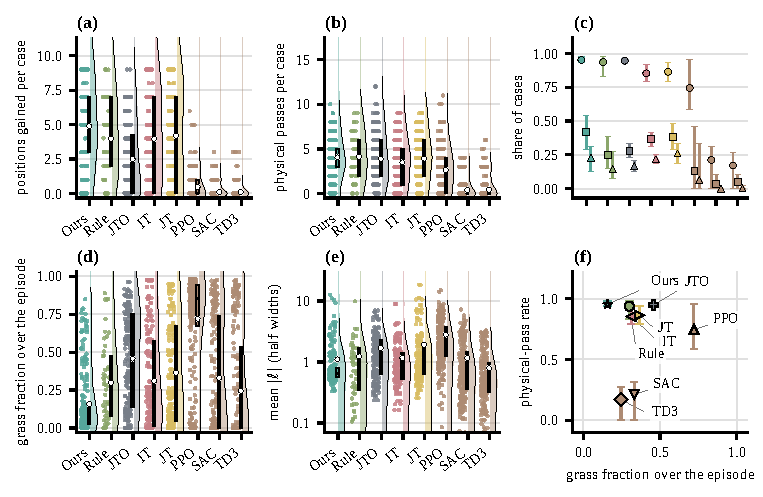
\includegraphics[width=0.80\textwidth]{figures/figure_main_endpoints.pdf}
\caption{Main comparison over the 48 shared cases.
(a) Positions gained per case. (b) Scored passing events per case.
(c) Share of cases reaching $P$ (circles), $E_{\mathrm{full}}$ (squares) and
$E_{\mathrm{race}}$ (triangles), with Wilson 95\,\% intervals.
(d) Grass fraction over the whole episode.
(e) Mean absolute lateral offset in road half widths. (f) Physical-pass rate
against grass fraction. Panels (a), (b), (d), (e): rainclouds (dots, box,
density).}
\label{fig:main_endpoints}
\end{figure*}

\subsection{Fleet size and the structure of the manoeuvre}
\label{sec:scale_and_manoeuvre}

Completion does not degrade with fleet size for the proposed controller: 57, 55,
59 and 58 of the sixty case-draw pairs at four, six, eight and ten vehicles. The
strict tier rises with the field instead, 18, 23, 29 and 31 of the same pairs,
and mean rank gain rises from 2.5 to 7.8 positions per case, because a larger
field offers both more vehicles to pass and more positions to gain. The
racing-rival tier does not follow it, 12, 14, 20 and 9: at ten vehicles the
passes that satisfy the strict tier are usually passes of a vehicle that has
already left the racing surface, and excluding those is what that tier adds. A
pass at ten vehicles also has to be made against nine opponents whose speeds
differ by less than 5~m/s, so the approach is longer and the hold window is more
often interrupted.

At eight vehicles the approach to a pass takes 125 steps and the alongside phase
111, against 98 and 163 for the rule expert: the rule expert reaches the vehicle
sooner and then spends half again as long beside it, and the side-by-side phase
is where contact and containment failures originate (Figs.~\ref{fig:snapshot}
and~\ref{fig:manoeuvre_profile}). Counted over all four fleet sizes, it also
spends 22 steps off the racing surface per completed pass against 66 for the
rule expert, 53 for the observer variant and 16 for the individual-transition
variant. The vehicle being passed is not passive: over the same pooled passes it
slows by at least 2~m/s inside the manoeuvre window in 8\,\% of them, against
24\,\% for the rule expert.
Table~\ref{tab:failure_modes} carries the failure profile: of the 27.8 cases
where the proposed controller misses $E_{\mathrm{full}}$, 17 lose the lead
before the window ends and 13.6 record contact, whereas the rule expert loses 27
cases to contact and 16 to stability over the same 48 cases.

\begin{figure*}[!t]
\centering
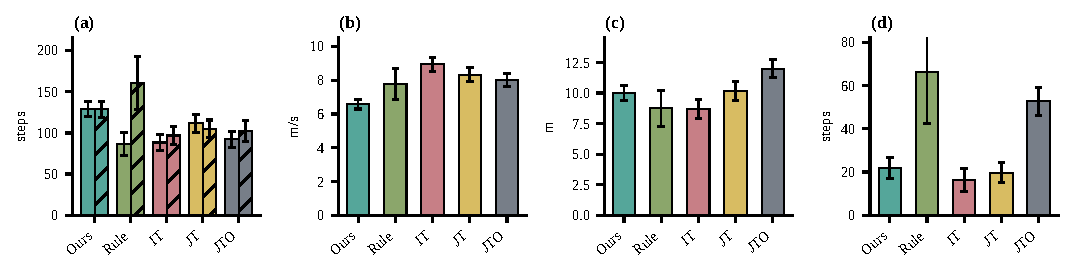
\includegraphics[width=\textwidth]{figures/figure_manoeuvre_profile.pdf}
\caption{Completed passes of the five structured controllers, pooled over the
four fleet sizes; means with the 95\,\% interval of the mean.
(a) Approach (solid) and alongside (hatched) phase. (b) Speed advantage
while alongside. (c) Closest centre-to-centre distance to the rival. (d) Steps
off the racing surface.}
\label{fig:manoeuvre_profile}
\end{figure*}

\begin{table}[!t]
\centering
\caption{Cases that fail a clause over the 48 cases of each method, averaged
over the draws of its recipe. Columns are not exclusive; a case with no
auditable pass counts under every column.}
\label{tab:failure_modes}
\footnotesize
\setlength{\tabcolsep}{3pt}
\begin{tabular}{lccccc}
\toprule
Method & no lead & contact & off track & stability & non-racing rival \\
\midrule
DNQ-DLC (ours)    & 17   & 13.6 & 3   & 4.6  & 5.6 \\
Rule expert       & 13   & 27   & 11  & 16   & 4 \\
DLC-IT            & 19.5 & 16.0 & 11.5 & 13.5 & 12.0 \\
DLC-JT            & 14.5 & 13.5 & 8.5 & 8.0  & 11.0 \\
DLC-JTO           & 15.0 & 14.5 & 8.0 & 5.0  & 12.0 \\
\bottomrule
\end{tabular}
\end{table}

\paragraph{Continuous-control families under retraining}
The three continuous-control families are a different operating regime rather
than a uniformly weaker one, and the retrained numbers sharpen the contrast that
the single-seed ones only suggested. PPO completes 35.8 physical passes of 48 on average,
fewer than any of the five structured controllers but nearly four times as many
as SAC, at a mean speed of 44.6~m/s while spending 72.1\,\% of the episode on
grass; SAC and TD3 complete 10.2 and 8.2 at 21.8 and 20.8~m/s and 33.1 and
24.5\,\% grass. What they do not convert is the pass: the strict tier falls to
6.4, 1.6 and 2.2 cases against the 20.2 of the proposed controller, and the
racing-rival tier to 3.2, 0.0 and 0.2 against 11.0.

\paragraph{Spread across training seeds}
The fifteen retrained agents disagree widely with one another, in both
directions. The best of them is a PPO seed that reaches the strict tier in 22
cases and the racing-rival tier in 16, above the proposed controller's five-draw
mean of 20.2 and 11.0 and, on the racing-rival tier, above its whole 6-to-15
range, while spending 73.4\,\% of the episode on grass at a mean lateral error of
2.70 half widths against 15.7\,\% and 1.11 for the proposed controller. The
best-contained of the fifteen is a TD3 seed at 2.7\,\% grass that completes no
pass at all. Either the endpoint count or the containment column can therefore
be attained without the other, which is why both are reported and why the paired
counts of Section~\ref{sec:main_comparison} are read against
Fig.~\ref{fig:main_endpoints}f.

\begin{figure*}[!t]
\centering
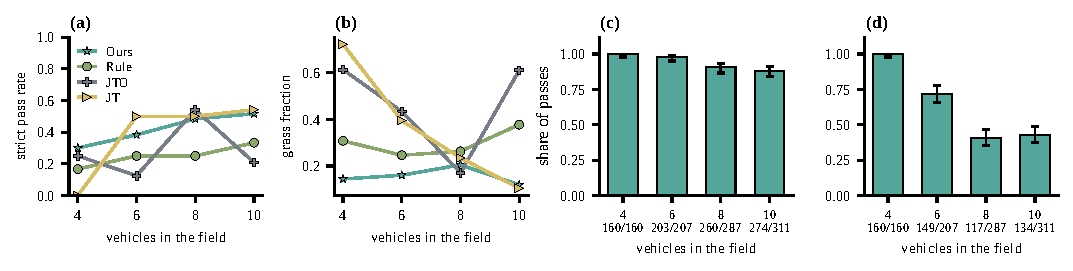
\includegraphics[width=0.97\textwidth]{figures/figure_scale_membership.pdf}
\caption{Fleet-size dependence of the four methods that complete most cases
(a, b) and membership of the overtaken vehicle under the proposed controller
(c, d). (a) Strict-tier rate. (b) Grass fraction over the whole episode.
(c) Share of passes whose partner entered the admitted set during the window.
(d) Share whose partner was still admitted at completion. Bars carry Wilson
95\,\% intervals and the raw counts.}
\label{fig:scale_membership}
\end{figure*}

\begin{figure}[!t]
\centering
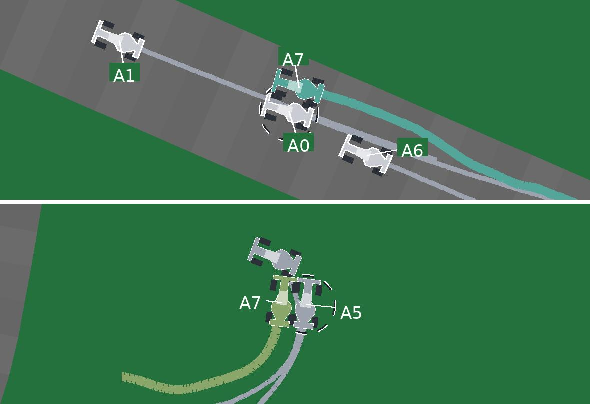
\includegraphics[width=0.86\columnwidth]{figures/figure_snapshot_m8_seed29.pdf}
\caption{Closest approach to a rival in one eight-vehicle case, episode seed 29:
the proposed controller at step 946 (top) and the rule expert at step 459
(bottom). The proposed controller admits rivals 0, 1 and 6 at its step. The
evaluated car A7 is drawn in its controller's colour, every car carries its
field index, and admitted rivals are in a lighter tint with a thicker outline.}
\label{fig:snapshot}
\end{figure}

\subsection{Mechanism evidence from the same runs}
\label{sec:mechanism_evidence}

The three claims of Section~\ref{sec:method} are measured from the runs that
produced Table~\ref{tab:main_comparison}, because the planner records its
admission decision, its imagined rollout and its candidate scores at every
step. Only one of the three is tested by removing the component: the admission
rule is replaced by two alternatives below. The imagined rollout and the quality
score are not, so for those two the evidence is the measured accuracy of the
rollout and the measured departure from the rule anchor, which show that both
are active in the executed decisions rather than that either is what produces
the endpoint.

\begin{table*}[!t]
\centering
\caption{Interaction-graph and planner statistics of the proposed controller,
means over the sixty cases at each fleet size. $|\mathcal N_t|$ and $K_t$ are
the exposed and admitted neighbour counts, $\pi$ and $\chi$ the shares of steps
that prune an exposed neighbour and change the admitted set, and $D$ the
distinct admitted neighbours per episode. $\varepsilon_1,\varepsilon_4$ are the
imagined ego-position errors in metres at horizons one and four;
$\rho_{\mathrm{p}},\rho_{\mathrm{s}},\rho_{\mathrm{o}}$ the shares of decision
steps with a feasible candidate, with the shield active, and leaving the rule
anchor.}
\label{tab:mechanism}
\footnotesize
\setlength{\tabcolsep}{7pt}
\begin{tabular}{@{}lcccccccccc@{}}
\toprule
Fleet size & $|\mathcal{N}_t|$ & $K_t$ & $\pi$ & $\chi$ & $D$ &
$\varepsilon_1$ & $\varepsilon_4$ & $\rho_{\mathrm{p}}$ &
$\rho_{\mathrm{s}}$ & $\rho_{\mathrm{o}}$ \\
\midrule
4  & 3.00 & 1.85 & 0.46 & 0.00 & 3.0 & 0.45 & 0.85 & 0.71 & 0.37 & 0.92 \\
6  & 5.00 & 2.30 & 1.00 & 0.02 & 4.7 & 0.46 & 0.98 & 0.67 & 0.42 & 0.92 \\
8  & 7.00 & 2.66 & 1.00 & 0.05 & 6.7 & 0.47 & 1.18 & 0.63 & 0.45 & 0.93 \\
10 & 9.00 & 2.85 & 1.00 & 0.06 & 8.3 & 0.46 & 1.05 & 0.74 & 0.35 & 0.92 \\
\bottomrule
\end{tabular}
\end{table*}

\paragraph{Size and composition of the interaction set}
Exposure grows linearly with the field while the admitted set saturates at the
slot budget of three: three, five, seven and nine opposing vehicles are exposed
at four, six, eight and ten vehicles, against 1.85, 2.30, 2.66 and 2.85
admitted. The admitted set is part of the observation the transition model is
trained on, not a filter on its input, and its composition changes: pruning
fires on 46\,\% of steps at four vehicles and on every step from six on, so the
exposed set is a strict superset of the admitted one in a dense field, and the
budget is filled on 54\,\% of steps at four vehicles against 91\,\% at ten
(Fig.~\ref{fig:mechanism_panel}a,b).

\paragraph{Choice of the admission rule}
\label{sec:selector_control}
Whether the ranking drives the effect was tested by re-packing the released
expert episodes offline under three rules at the same budget of three slots: the
interaction ranking, the three nearest opponents, and the first three opponents
in identity order. The three datasets therefore share the episode plan, the
expert actions, the rewards and the risks exactly and differ only in the packed
slots (maximum slot difference 2.0, behaviour difference 0.0 over 352000
transitions). Retrained under the identical recipe with a single-member model,
and evaluated on the same 48 cases, the interaction ranking reaches the strict
tier in 21 cases against 17
for the nearest rule and 15 for the fixed identity window, and the racing-rival
tier in 14, 7 and 9. The rank gain falls from 4.96 to 4.52 and 2.73 positions
per case, the whole-episode grass fraction rises from 0.179 to 0.238 and 0.376,
and the mean lateral error from 0.79 to 0.97 and 2.42 half widths. A window that
is never re-selected is also behind on the physical pass $P$, 36 of 48 against
46, a paired difference of $-10$ with a bootstrap interval excluding zero.
Proximity alone carries the pass, which the nearest rule shows by matching 46 of
48 and leading on $E_{\mathrm{pass}}$, 27 against 24, but not the later
conditions: it loses more of those passes to the on-track and stability clauses,
so the strict tier falls to 17 against 21 and the racing-rival tier to 7 against
14. At that tier the two rules disagree in 13 cases, and the nearest rule is
ahead in 3 of them and behind in 10.

\paragraph{Membership of the overtaken vehicle}
Reading the same runs by event rather than by case makes set membership
measurable: the five draws together yield 965 auditable passing events, and the
partner is inside the admitted set somewhere in the window in 897 of them,
93.0\,\% (Wilson [91, 94]): 160 of 160 at four vehicles, 203 of 207 at six, 260
of 287 at eight and 274 of 311 at ten (Fig.~\ref{fig:scale_membership}c). The
composition also changes, on average 3.5 times within the window (4.9 at eight
vehicles, 4.4 at ten), against 0.006 at four. Once the ego has crossed, the
partner is behind it and no longer closing, so the selector releases it: it is
still admitted at completion in 41\,\% of eight-vehicle and 43\,\% of ten-vehicle
passes, against 100\,\% at four (Fig.~\ref{fig:scale_membership}d). Holding it
beyond the crossing would spend a slot on a vehicle that is already behind the
evaluated one, so the evaluated configuration releases it.

\paragraph{Accuracy of the imagined rollout}
The planner scores candidates on a four-step horizon and the imagined ego
position is 0.45 to 0.47~m from the realized trajectory after one step and 0.85
to 1.18~m after four, with mean speed errors of 0.73 to 0.85~m/s at one step and
1.59 to 1.98~m/s at four. The four-step error is about a quarter of a
vehicle length over the $0.08$~s the four-step ranking spans.

\paragraph{Quality guidance and the rule anchor}
The planner carries a rule-based anchor and departs from it on 92--93\,\% of
decision steps, by a score margin that averages 134 to 237 units, so the
quality-guided ranking rather than the anchor sets the executed action almost
everywhere. The anchor is $c_{\rm anchor}$ of (\ref{eq:candidate_pool}), a
rule-based telemetry gate of the same family as the rule-expert reference, so
the ranking overrides that expert's own command on almost every step rather
than replaying it.

\paragraph{Residual contribution of the recovery shield}
The shield is active on 35--45\,\% of steps, the planner has a feasible candidate
on 63--74\,\%, the guard's own trigger fires on 13--15\,\%, and on 26--37\,\% of
steps the escalated pool holds no feasible manoeuvre, so the geometric recovery
controller drives. Disabling the shield over the same five draws leaves the
strict tier where it is, 20.6 cases against 20.2, and the containment lead is
intact: the whole-episode grass fraction rises from 0.157 to 0.169 but stays
below every draw of every comparator, whereas completion falls from 45.8 to 44.6
cases and the racing-rival tier from 11.0 to 8.8
(Table~\ref{tab:main_comparison}). The shield therefore secures the last of the
clause of the graded endpoint, that the vehicle being passed is still racing, together
with two completions, rather than the strict tier itself.

\begin{figure*}[!t]
\centering
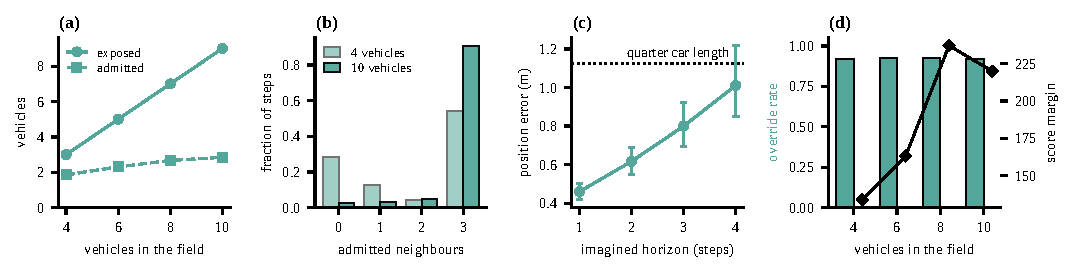
\includegraphics[width=\textwidth]{figures/figure_mechanism_panel.pdf}
\caption{Controller-internal signals of the proposed controller, from the same
runs as Table~\ref{tab:main_comparison}. (a) Exposed and admitted neighbours
against field size. (b) Admitted count at the smallest and largest fields.
(c) Imagined position error against horizon. (d) Override rate (bars) and mean
score margin (line).}
\label{fig:mechanism_panel}
\end{figure*}

\subsection{Failure cases and boundaries}
\label{sec:failures}

In two of the 48 runs of the submitted draw of the proposed controller, at six
vehicles seed 32 and at eight vehicles seed 22, the evaluated vehicle covers 0.16
and 0.23 of a lap with no auditable passing event, confined behind a slower
vehicle early and never recovering the speed to open a gap. Both count as failures in every rate of
Table~\ref{tab:main_comparison}, but they do not limit the strict rate at ten
vehicles, where every case completes and the limit is the hold window,
interrupted more often as the field grows.

Two boundaries limit what the tables support. The strict tier is an audit
criterion, not a validated safety limit, and the references are not trained to
convergence, so the comparison characterizes the systems as evaluated rather
than ranking algorithms under optimal training. Nothing here is a claim about a
physical vehicle.

\section{Conclusion and Future Work}
This paper addressed closed-loop overtaking in multi-vehicle autonomous racing,
where the opponent that constrains a pass can change while the pass is under way.
DNQ-DLC selects the currently relevant opponents from each real observation,
predicts their short-horizon interaction with candidate ego actions through an
action-conditioned graph world model, and ranks candidates by progress together
with containment, interaction quality, boundary risk and uncertainty before
committing the first action.

The evaluation compared the complete controller with rule-based and learned
references over 48 shared cases per method. Averaged over the five
draws of its recipe the controller completes 45.8 of 48 cases and reaches the
strict tier in 20.2 of them, against 12 for the rule expert and 13.5 to 18.5 for
the three world-model variants. What separates it from the rule expert is not the
number of passes, which the expert matches, but the fraction of those passes that
survive the containment and stability conditions. The result is bounded in three
ways. The shield remains active on 30 to 46\,\% of steps, and removing it leaves
the strict tier unchanged while costing the racing-rival tier and two
completions, so the endpoint that depends on it is the last clause of the graded
endpoint rather than the strict tier. The continuous-control references bound
what PPO, SAC and TD3 reach at a five-hundred-thousand-step budget under five
seeds each; the best of the fifteen seeds passes the proposed controller on the
strict tier while spending 73.4\,\% of the episode on grass. And the strict-tier
count of the five draws spans 14 to 26 cases, so the size of the margin over the
rule expert belongs to the draw, which is why that endpoint is reported as
counts and intervals. Every learned row of
Table~\ref{tab:main_comparison} is the mean over the draws of its recipe, so no
column depends on the choice of draw. Future work will keep
the representation slots aligned with vehicle identity as the ranking changes,
drive the shield activation toward zero, and move the planner to closed-course
vehicle experiments.

\section*{Data and Code Availability}
The simulator, controller, evaluation and analysis code, the checkpoints, the
configurations and the per-case evaluation and audit tables behind
Section~\ref{sec:experiments} are at
\url{https://github.com/chocho2222/DNQ-DLC}, released as the content-addressed
snapshot \emph{tits-2026-09-29} (1755 files, 97.1 MB); the recorded trajectories
are 8.5~GB for the retrained baselines alone and are not part of it. Every number
in Section~\ref{sec:experiments} is computed from those tables. The snapshot
adds, relative to the earlier one, the fifteen strict continuous-control
checkpoints with their tier and containment audits, the further
transition-model draws, the five-draw and fused-ensemble runs, the held-out
prediction and recovery-deferral checks, the re-run of the admission-rule
control under the corrected planner, and the tables behind
Figs.~\ref{fig:manoeuvre_profile} and~\ref{fig:snapshot}. The digest, SHA-256 over sorted
$\langle$root$\rangle$/$\langle$path$\rangle$:$\langle$digest$\rangle$ lines, is
\texttt{2d3af4413d04ff96bfd1a85bdc8c9d1b}\newline\texttt{57f48f2a40b3cdac46dd8913225ece98}.
Recomputing it over a local copy confirms the copy is the evaluated one; the
audit roots are listed in the released manifest.

% Funding, acknowledgments, author contributions, affiliations, ORCID
% identifiers, and corresponding-author information are provided separately.

\bibliographystyle{IEEEtran}
\bibliography{references}

\end{document}
